%==============================================================================
%  Acousto-Cymatic Phase-Change Memory (ACPCM)
%  A speculative ("idea paper") theoretical framework, arXiv preprint style.
%
%  Compile (recommended, self-contained engine):
%      tectonic main.tex
%  or with a full TeX Live:
%      pdflatex main && pdflatex main
%
%  No external .bib needed: the bibliography is embedded (thebibliography).
%  Every reference below was independently verified (Crossref / publisher /
%  arXiv / ADS) during preparation; see README.md for the audit trail.
%==============================================================================
\documentclass[11pt]{article}

% ---- Page geometry: arXiv-like single column -------------------------------
\usepackage[letterpaper,margin=1in]{geometry}

% ---- Encoding & fonts (Times-like, the classic preprint look) --------------
% fontenc/inputenc only matter for the pdflatex fallback; under XeTeX/LuaTeX
% (tectonic) newtx uses fontspec and inputenc would warn, so guard them.
\usepackage{iftex}
\ifPDFTeX
  \usepackage[T1]{fontenc}
  \usepackage[utf8]{inputenc}
\fi
% Load amsmath/amsthm first; do NOT load amssymb (its \Bbbk clashes with
% newtxmath, which already provides the AMS symbol set we use).
\usepackage{amsmath}
\usepackage{amsthm}
\usepackage{newtxtext,newtxmath}
\usepackage{microtype}
\setlength{\emergencystretch}{1em} % relieve minor overfull boxes

% ---- Units -----------------------------------------------------------------
\usepackage{siunitx}
\sisetup{detect-all=true}

% ---- Graphics, color, tables -----------------------------------------------
\usepackage{graphicx}
\usepackage{xcolor}
% Plain-academic palette: monochrome. Headings/links black; figures in grayscale;
% callout boxes have no fill (white) and a thin near-black rule.
\definecolor{acpcmblue}{HTML}{000000}
\definecolor{acpcmteal}{HTML}{595959}
\definecolor{acpcmgray}{HTML}{4D4D4D}
\definecolor{warnbg}{HTML}{FFFFFF}
\definecolor{warnrule}{HTML}{1A1A1A}
\usepackage{booktabs}
\usepackage{array}
\usepackage{tabularx}
\usepackage{caption}
\captionsetup{font=small,labelfont=bf,labelsep=period}

% ---- Lists, boxes, headers -------------------------------------------------
\usepackage{enumitem}
\usepackage[most]{tcolorbox}
\usepackage{fancyhdr}
\usepackage{titlesec}
\usepackage{authblk}

% ---- Diagrams --------------------------------------------------------------
\usepackage{tikz}
\usetikzlibrary{arrows.meta,positioning,calc,shapes.geometric,backgrounds,fit,decorations.pathmorphing,patterns}
\usepackage{pgfplots}
\pgfplotsset{compat=1.18}
\usepackage{placeins} % \FloatBarrier - keep floats from drifting across sections

% ---- Hyperlinks (load late, then cleveref last) ----------------------------
\usepackage[colorlinks=true,allcolors=acpcmblue,breaklinks=true]{hyperref}
\usepackage{cleveref}
\crefname{prediction}{Prediction}{Predictions}
\Crefname{prediction}{Prediction}{Predictions}
\crefname{assumption}{Assumption}{Assumptions}
\Crefname{assumption}{Assumption}{Assumptions}

% ---- Section styling --------------------------------------------------------
\titleformat{\section}{\normalfont\large\bfseries\color{acpcmblue}}{\thesection}{0.6em}{}
\titleformat{\subsection}{\normalfont\normalsize\bfseries\color{black}}{\thesubsection}{0.6em}{}

% ---- Running header ---------------------------------------------------------
\pagestyle{fancy}
\fancyhf{}
\renewcommand{\headrulewidth}{0.4pt}
\fancyhead[L]{\footnotesize\itshape Acousto-Cymatic Phase-Change Memory}
\fancyhead[R]{\footnotesize\thepage}
\fancypagestyle{plain}{\fancyhf{}\fancyhead[R]{\footnotesize\thepage}\renewcommand{\headrulewidth}{0pt}}

% ---- Epistemic-status callout box ------------------------------------------
\newtcolorbox{epistemic}[1][]{
  enhanced, breakable, sharp corners,
  colback=warnbg, colframe=warnrule, boxrule=0.8pt,
  left=8pt,right=8pt,top=6pt,bottom=6pt,
  fonttitle=\bfseries, coltitle=warnrule,
  title=Epistemic status, #1
}

% ---- Theorem-like environments ---------------------------------------------
\theoremstyle{definition}
\newtheorem{prediction}{Prediction}
\newtheorem{assumption}{Assumption}

% ---- Title metadata ---------------------------------------------------------
\title{\bfseries\color{acpcmblue}\Large Acousto-Cymatic Phase-Change Memory:\\[2pt]
A Speculative Theoretical Framework for High-Density Data Storage\\ in Confined Aqueous Media}

\author{Sahar Barak\thanks{Correspondence: \texttt{hi@saharbarak.dev}.}}
\affil{Independent Researcher}

\date{\small Preprint - \today \\[2pt] \emph{Speculative ``idea paper'' (cf.\ \texttt{physics.pop-ph} / \texttt{cs.ET}).}}

%==============================================================================
\begin{document}
\maketitle
\thispagestyle{plain}

%------------------------------------------------------------------ Abstract
\begin{abstract}
\noindent
As conventional magnetic and solid-state storage technologies approach fundamental
physical scaling limits - most notably the superparamagnetic limit~\cite{charap1997,wellermoser1999} - new
architectures are sought to meet global data demand. This paper proposes, as a
deliberately speculative thought experiment, a data-storage architecture we call
\emph{Acousto-Cymatic Phase-Change Memory} (ACPCM). By drawing engineering analogies
from Heat-Assisted Magnetic Recording (HAMR)~\cite{kryder2008hamr}, three-dimensional
charge-trap flash~\cite{white2000sonos,tanaka2007bics}, megahertz acoustic
holography~\cite{melde2016holograms}, and scientific data
sonification~\cite{hermann2011handbook}, we sketch a method for encoding digital data
into the physical topology of a confined, rapidly frozen aqueous ``pod.'' In the
proposal, data is encoded as acoustic frequencies, organized into a three-dimensional
grid by cymatic pressure nodes, and locked into a solid lattice by a HAMR-style
``broadcast-and-freeze'' phase transition; read-back is designed around established
megahertz acoustic holography and neural-network field inversion, isolating the
speculative burden on the write side. We are explicit throughout about which
ingredients are established physics and which are contested or non-mainstream
(``water memory,'' structured-water chains, and W.~Russell's octave cosmology). Rather
than asserting feasibility, we cast the architecture as a set of falsifiable predictions
and identify the physical obstacles - above all the energetics, lattice distortion, and
the ${\sim}50$\,fs memory loss and picosecond reorganization of the hydrogen-bond
network~\cite{cowan2005water} - that would have to be overcome for any such scheme to be
viable. We make the reckoning quantitative: granting even the contested ``structured-water''
figures their own most favourable numbers, the binding constraint is not molecular packing
but the \emph{acoustic diffraction limit of the read path} (in ice, not water), which caps a
realistic megahertz-addressed pod at ${\sim}10^{4}$--$10^{5}$ bits per cubic millimetre -
some 9--14 orders of magnitude below the molecular and structured-water ceilings - while the
energy to freeze a bit lands orders of magnitude above incumbent
storage~\cite{horowitz2014energy}; against established archival media such as 5D
fused-silica glass~\cite{zhang2014glass} and DNA~\cite{erlich2017fountain}, ACPCM is, on
these numbers, uncompetitive. We further locate the proposal against the
\emph{sonocrystallization} literature~\cite{zhang2021uafmech}: ultrasound demonstrably imprints
structure on freezing ice, but through \emph{cavitation} - a stochastic, pattern-destroying
mechanism - so the architecture's cheapest test is at risk of a misleading positive and must
control for it, while the one genuinely buildable variant (acoustically assembling seeded
scatterers and locking them by solidification, already demonstrated~\cite{melde2023assembly})
records particle positions rather than the water field itself. Finally we sketch the pivot
that lets the idea stand as a \emph{device} rather than a high-density medium: built from
directional (freeze-cast) solidification below the Mullins--Sekerka instability, seeded
acoustic scatterers, and millitesla magnetic grain orientation - each demonstrated in
isolation - and pitched not on density but on substrate cost, non-toxicity, and recyclability
in environments where cold is free. The contribution is a conceptual synthesis, a
quantitative bound, a device-shaped operating point, and a research agenda, \emph{not} a
validated device.
\end{abstract}

\vspace{2pt}
\noindent\textbf{Keywords:} unconventional computing; acoustic holography; acoustofluidics;
phase-change media; ice nucleation; data sonification; speculative storage architectures.

%------------------------------------------------------------------ Epistemic status box
\begin{epistemic}
This is a \textbf{speculative theoretical proposal}, written in the spirit of an
``idea paper.'' It combines \emph{established} engineering mechanisms with
\emph{contested or refuted} premises, and it should be read as a hypothesis generator,
not as a report of a working device or of accepted science.
\begin{itemize}[leftmargin=1.4em,nosep]
  \item \textbf{Established} (well supported in the literature): the superparamagnetic
  limit and HAMR~\cite{charap1997,wellermoser1999,kryder2008hamr,challener2009};
  3D charge-trap flash~\cite{white2000sonos,tanaka2007bics,goda2020}; chalcogenide
  phase-change memory~\cite{ovshinsky1968,wuttig2007pcm,raoux2010pcm}; passive
  acoustic-hologram phase plates and acoustofluidic
  patterning~\cite{melde2016holograms,marzo2015holographic,rufo2022acoustofluidics};
  deep-learning acoustic-hologram synthesis~\cite{lin2021dlholograms}; and data
  sonification as a methodology~\cite{kramer1999nsf,hermann2011handbook}.
  \item \textbf{Contested / minority view}: ``exclusion-zone / fourth-phase'' structured
  water~\cite{pollack2013fourth} (the interfacial effect is real but its structural
  interpretation is disputed~\cite{elton2020ez}); quantum coherence in microtubules
  (Orch-OR)~\cite{hameroff2014orchor}, challenged on decoherence
  grounds~\cite{tegmark2000decoherence}.
  \item \textbf{Refuted / pseudoscientific} (used here only as historical or motivational
  framing, \emph{not} as evidence): ``water memory''~\cite{benveniste1988}, which an
  on-site investigation found did not survive blinding~\cite{maddox1988} and which later
  revivals~\cite{montagnier2009} did not reproduce; and W.~Russell's octave periodic
  system~\cite{russell1926universalone}.
\end{itemize}
A claim's appearance in this paper is \emph{not} an endorsement of its validity. Crucially,
the established citations ground only their own subsystems; none of them lends support to
the central acousto-cymatic conjecture, which is ours and is clearly labelled as
speculation throughout. \Cref{sec:limits} and \cref{tab:status} make the dependencies
explicit.
\end{epistemic}

%================================================================== 1. Introduction
\section{Introduction}
\label{sec:intro}

The data-storage industry is constrained by a set of competing requirements - high areal
density (which demands small grains), thermal (bit) stability (which demands high magnetic
anisotropy), and writeability (which demands a switching field a head can actually
supply) - that become mutually exclusive as bits shrink; in the later literature this is
often called the \emph{recording trilemma}~\cite{wellermoser1999}. The underlying physics
is thermodynamic: as a grain's volume $V$ shrinks, its anisotropy energy $K_{\mathrm{u}}V$
falls toward the thermal energy $k_{\mathrm{B}}T$, and once the stability ratio
$K_{\mathrm{u}}V/k_{\mathrm{B}}T$ drops below ${\sim}40$--$60$ the magnetization reverses
spontaneously - the \emph{superparamagnetic limit}, whose onset Charap, Lu, and He first
projected for thin-film media~\cite{charap1997} and which Weller and Moser analyzed in its
modern form~\cite{wellermoser1999}.\footnote{Their projected areal-density upper bound of
${\sim}36$\,Gbit/in$^2$ for longitudinal media was later surpassed by media engineering and
perpendicular recording; we cite it as a projected estimate, not a proven wall.}
The industry's response, \emph{Heat-Assisted Magnetic Recording} (HAMR), uses a near-field
plasmonic transducer to heat a high-anisotropy medium close to its Curie temperature for
well under a nanosecond, transiently collapsing its coercivity so a modest field can write
a bit, after which rapid cooling ``freezes'' the magnetization into a thermally stable
state~\cite{kryder2008hamr}; the near-field-transducer write process has been demonstrated
experimentally~\cite{challener2009} and HAMR is now shipping commercially.

In parallel, solid-state drives escaped planar scaling by going vertical: 3D NAND with
\emph{charge-trap flash} (CTF) stores charge in a discrete, electrically insulating
silicon-nitride layer rather than a continuous conductive floating gate, so a single local
defect leaks only its neighborhood rather than draining a shared
pool~\cite{white2000sonos}; the move to stacked, ``punch-and-plug'' vertical strings
decoupled density from lithography~\cite{tanaka2007bics,goda2020}.

This paper asks a deliberately unconventional question: \emph{what if the two core ideas
behind these technologies - rapid state-change writing (HAMR) and microscopic spatial
isolation (CTF) - were applied to an exotic medium, namely water frozen on demand?} Liquid
water is, on its face, the worst imaginable storage medium: its hydrogen-bond network loses
memory of its configuration within ${\sim}50$\,fs and fully reorganizes on a picosecond
timescale~\cite{cowan2005water}, so any imprint in the \emph{liquid} is erased almost
immediately. Our proposal confronts this directly by never trying to store information in
the liquid: information exists only fleetingly as a broadcast acoustic field and is
committed to memory by an \emph{instantaneous phase change} into ice, in loose analogy to
HAMR's heat-then-quench write cycle~\cite{kryder2008hamr} and to chalcogenide phase-change
memory's melt--quench amorphization~\cite{ovshinsky1968,wuttig2007pcm}.

We stress at the outset (and repeat in \cref{sec:limits}) that several premises in the
draft framing of this idea - ``water memory,'' long-lived ``structured-water'' chains, and
an octave-based re-mapping of the periodic table - are \emph{not} part of accepted physics
or chemistry; the first was specifically investigated and not
reproduced~\cite{maddox1988,benveniste1988}. We include them transparently, label their
status, and engineer the architecture so that the refuted ideas carry no logical load. The
intended contribution is a clean conceptual synthesis across fields that are rarely
discussed together, plus an explicit map of where the idea would break.

\paragraph{Where this sits among unconventional storage.}
The search for post-magnetic archival media is well populated, and ACPCM should be judged
against it. \emph{5D optical data storage} writes birefringent nanogratings into fused
silica with a femtosecond laser - three spatial coordinates plus slow-axis orientation and
retardance - with a peer-reviewed room-temperature decay time of order $10^{20}$\,years and
thermal stability to \qty{1000}{\celsius}~\cite{zhang2014glass}, and demonstrated
high-speed writing toward hundreds-of-terabytes-per-disc capacities~\cite{lei2021optica}.
\emph{DNA data storage} encodes bits in synthesized oligonucleotides: from the first
megabit-scale demonstrations~\cite{church2012dna,goldman2013dna} to a coding density of
$1.57$~bits/nucleotide and an experimentally realized
$215$~PB/g~\cite{erlich2017fountain}, with random access at the
${\sim}200$\,MB scale~\cite{organick2018random} and a molecular ceiling near
$10^{18}$\,bytes/mm$^{3}$~\cite{ceze2019molecular}. \emph{Volume holographic storage}
records data as superimposed interference gratings with a theoretical ceiling of order
$V/\lambda^{3}$~\cite{heanue1994holographic,coufal2000holographic}. Each is mature or at
least experimentally grounded; ACPCM is far more speculative than any of them, and
\cref{sec:capacity} places it on the same axes so the comparison is explicit rather than
rhetorical.

\paragraph{Contributions.}
\begin{enumerate}[leftmargin=1.6em,nosep]
  \item A subsystem-by-subsystem architecture (medium, format, write, read) that
  transposes HAMR and CTF design principles onto a rapidly frozen aqueous medium
  (\cref{sec:medium,sec:format,sec:write,sec:read}).
  \item An explicit \emph{epistemic ledger} (\cref{tab:status}) separating established
  mechanisms from speculative ones, so the proposal cannot be mistaken for a validated
  device and so that mainstream citations are not laundered into supporting fringe claims.
  \item A \emph{quantitative reckoning} (\cref{sec:capacity}) that derives the achievable
  density from the acoustic diffraction limit, takes the contested structured-water capacity
  figures at face value to show what would be required, and benchmarks the resulting density
  and energy-per-bit against 5D glass, DNA, and incumbent semiconductor storage
  (\cref{tab:comparators}).
  \item A set of falsifiable predictions and order-of-magnitude obstacles
  (\cref{sec:predictions,sec:limits}) that define what an experimental test would have to
  measure.
\end{enumerate}

%================================================================== System overview figure
\begin{figure}[t]
\centering
% NB: section refs inside these tight TikZ nodes use the compact \S\ref idiom
% on purpose (cleveref's "Section N" is too wide for the boxes); the body prose
% uses \cref throughout. Deliberate, applied consistently within this figure.
\begin{tikzpicture}[
  font=\small,
  node distance=6mm,
  stage/.style={draw=acpcmblue,thick,rounded corners=2pt,fill=acpcmblue!6,
    align=center,minimum height=10mm,inner sep=4pt,text width=24mm},
  io/.style={draw=acpcmteal,thick,rounded corners=8pt,fill=acpcmteal!10,
    align=center,minimum height=10mm,inner sep=4pt,text width=16mm},
  arr/.style={-{Stealth[length=2.4mm]},acpcmgray,thick}
]
% Write path
\node[io] (bits1) {Digital\\bits};
\node[stage,right=of bits1] (son) {Elemental\\sonification\\(\S\ref{sec:write})};
\node[stage,right=of son] (cym) {Cymatic\\format grid\\(\S\ref{sec:format})};
\node[stage,right=of cym] (freeze) {Broadcast\\\& freeze\\(\S\ref{sec:write})};
\node[io,right=of freeze] (ice) {Frozen\\pod};
\draw[arr] (bits1) -- (son);
\draw[arr] (son) -- (cym);
\draw[arr] (cym) -- (freeze);
\draw[arr] (freeze) -- (ice);
% Read path (below)
\node[stage,below=10mm of son] (pulse) {MHz acoustic\\pulse\\(\S\ref{sec:read})};
\node[stage,below=10mm of cym] (holo) {Scattered 3D\\pressure field};
\node[stage,below=10mm of freeze] (unet) {Hydrophone\\+ U-Net\\decode};
\node[io,below=10mm of bits1] (bits2) {Digital\\bits};
\draw[arr] (ice.south) |- (pulse.east);
\draw[arr] (pulse) -- (holo);
\draw[arr] (holo) -- (unet);
\draw[arr] (unet) -- (bits2);
% labels
\node[acpcmblue,font=\footnotesize\bfseries,above=1mm of cym] {WRITE PATH};
\node[acpcmteal,font=\footnotesize\bfseries,below=1mm of holo,yshift=-7mm] {READ PATH};
\end{tikzpicture}
\caption{End-to-end ACPCM data path. The write path encodes bits as acoustic tones,
imposes a cymatic addressing grid, and commits the field to a solid lattice by freezing.
The read path probes the frozen pod with a megahertz pulse, treats the ice topology as an
acoustic phase plate, and decodes the scattered field with a neural network. The read path
and the write \emph{actuation} reuse established techniques; the speculative weight is
isolated in the freeze step (\cref{as:commit}). Each block's epistemic status is given in
\cref{tab:status}.}
\label{fig:overview}
\end{figure}

%================================================================== 2. Medium
\section{The storage medium: confined aqueous ``pods''}
\label{sec:medium}

For water to act even momentarily as an addressable medium, it cannot be a bulk volume.
In bulk liquid, distinct driving frequencies superpose and produce beat phenomena, so
independently addressed ``cells'' would modulate and erase one another (crosstalk). The
proposal therefore confines the medium to discrete \emph{pods} that physically isolate
addressable regions - an acoustic analogue of CTF's discrete charge traps, where isolation,
not bulk capacity, is the design goal~\cite{white2000sonos}.

A note on scale is needed up front, because it disciplines everything that follows. The
addressing grid is drawn by a megahertz field, so the smallest feature it can write or read
is set by that field's wavelength: at \qtyrange{5}{50}{\mega\hertz} the half-wavelength in
water is ${\sim}\qtyrange{15}{150}{\micro\meter}$ (\cref{sec:diffraction}). A pod must
therefore be \emph{at least} a few wavelengths across to host an internal grid at all - of
order \qtyrange{0.1}{1}{\milli\meter}, not sub-micron. We retain ``microscopic'' only in the
loose sense of sub-millimetre; the isolation in \cref{as:confine} is between neighbouring
pods in an addressed array, not within a single nanoscale cell. Any nanometre-scale
structure invoked below (microtubule water, structured-water ``pearls'') is therefore
\emph{motivational only} and explicitly \emph{not} the addressed unit - a point the capacity
reckoning of \cref{sec:capacity} makes quantitative.

\begin{assumption}[Confinement enables isolation]\label{as:confine}
Sub-millimetre pod confinement suppresses inter-pod acoustic crosstalk enough that
independently addressed pods do not annihilate one another during the write window.
\end{assumption}

As biological \emph{motivation only}, we note the recurring (and contested) claim that
cytoskeletal microtubules - hollow cylinders with an inner diameter of order
\qty{15}{\nano\meter} - might shield ordered internal water from thermal noise, a premise of
the Orch-OR quantum-biology hypothesis~\cite{hameroff2014orchor}. (This is a nanometre-scale
intuition pump, four orders of magnitude below the sub-millimetre addressed pod above; we
borrow only the \emph{qualitative} notion that confinement protects order.) That premise is itself
disputed: Tegmark's decoherence estimates put any quantum coherence in warm, wet
microtubules many orders of magnitude below cognitive
timescales~\cite{tegmark2000decoherence} (a critique that proponents have in turn disputed
on modelling grounds). We therefore use microtubules strictly as an intuition pump for
``confinement protects order'' and assert nothing about biological memory. Likewise, the
notion of long-lived spherical ``water pearls'' or ``trimmed chains'' as information
carriers belongs to the structured-water literature~\cite{pollack2013fourth}; the
underlying interfacial exclusion-zone effect is real and replicated, but its
``fourth-phase'' structural interpretation is a contested minority view that conventional
mechanisms may explain better~\cite{elton2020ez}. In ACPCM such structures, if they exist
at all, are relevant only \emph{after} freezing has removed the liquid's thermal lability,
not before.

%================================================================== 3. Format
\section{Format: a cymatic cylinder--head--sector grid}
\label{sec:format}

Conventional drives impose logical structure - tracks and sectors mapped to logical block
addresses - onto a physical medium. ACPCM proposes to impose this structure
\emph{acoustically}. Using megahertz ultrasound projected into the pod, intersecting
wavefronts establish a three-dimensional pattern of standing-wave nodes (pressure minima)
and antinodes. The nodal surfaces are intended to act as ``sector walls,'' partitioning the
pod into addressable voxels with definite spatial coordinates.

The \emph{patterning of matter by sound} is established physics. Since Faraday it has been
known that vibrating surfaces and liquid layers drive particles into ordered
figures~\cite{faraday1831}; modern acoustofluidics uses MHz standing waves to focus,
separate, and trap particles and cells at radiation-force nodes~\cite{rufo2022acoustofluidics},
down to one cell per well~\cite{collins2015saw}, and single-sided holographic arrays form
programmable ``acoustic tweezers'' and vortex traps that levitate and manipulate discrete
objects~\cite{marzo2015holographic,marzo2018vortices}. Passive acoustic-hologram phase
plates can sculpt remarkably intricate 3D pressure landscapes from a single
transducer~\cite{melde2016holograms,memoli2017bricks}.

\begin{epistemic}[colback=warnbg]
The \emph{spatial arrangement of discrete particles, droplets, or cells at acoustic nodes}
is established and reproducible (\cref{fig:pod}) - but it is transient (it lasts only while
the field is on) and it organizes \emph{pre-existing objects}. The stronger claim that such
fields coerce \emph{water molecules themselves} into a persistent ``supramolecular
network'' - sometimes labelled ``molecular cymatics'' - is \textbf{not} established: it has
no accepted mechanism and no primary literature specifically linking acoustic-field forcing
to supramolecular water ordering (the structured-water
literature~\cite{pollack2013fourth,elton2020ez} concerns interfacial proximity, not
acoustic induction), and liquid-water hydrogen bonds relax in
picoseconds~\cite{cowan2005water}. It is treated here purely as a hypothesis
(\cref{as:cymgrid}), and must not be confused with the established assembly result.
\end{epistemic}

\begin{assumption}[Cymatic addressing]\label{as:cymgrid}
A megahertz standing-wave field can define stable, reproducible nodal boundaries at the
length scale of the intended voxels, and these boundaries survive the freezing transition
well enough to serve as a read-time coordinate system.
\end{assumption}

\subsection{Two-axis addressing: slice into discs, then encode each disc}
\label{sec:biaxial}
We separate \emph{addressing} from \emph{encoding} by superposing two orthogonal acoustic
fields of very different scale - directly analogous to a hard drive's split between the
coarse mechanical track/cylinder geometry and the fine, high-frequency bit cells written
along a track.

\begin{enumerate}[leftmargin=1.6em,nosep]
  \item \textbf{A low-frequency axial ``slicing'' wave (the disc former).} A single
  longitudinal standing wave along the pod's $z$-axis, at the \emph{low} end of the band,
  partitions the pod into a stack of parallel nodal planes spaced by $\lambda_z/2$. Its
  pressure antinodes define a register of flat ``discs'' (the platter/cylinder analogue) -
  a small number of robust, widely spaced, easily resolved layers. Because $\lambda_z$ is
  large, these boundaries are the most likely structure to \emph{survive freezing}
  (\cref{sec:limits}) and so anchor the read-time coordinate system.
  \item \textbf{An orthogonal directional ``encoding'' wave (the in-disc data).} Within each
  disc, a transverse, higher-frequency, \emph{travelling-or-standing} field projected along
  $(x,y)$ writes the payload: the fine pressure pattern in the plane of a disc is the data,
  the multi-tone codebook of \cref{sec:write} modulating amplitude and phase across the
  disc. The encoding wave rides at the fine end of the resolution budget; the slicing wave
  guarantees that the decoder always knows \emph{which} disc a given fine feature belongs
  to.
\end{enumerate}

The two axes are deliberately decoupled in frequency so that the coarse layer index is
robust even where the fine payload is degraded - a graceful-degradation property borrowed
from how a drive can still seek a track whose individual bits are marginal. It also makes
the diffraction budget legible: the disc count is set by $\lambda_z$, the in-disc bit count
by the transverse wavelength, and the achievable product is bounded in \cref{sec:capacity}.

\begin{assumption}[Separable addressing]\label{as:biaxial}
A coarse axial standing wave and a fine transverse field can be imposed simultaneously
without the strong (low-frequency) former corrupting the weak (high-frequency) payload, and
the disc boundaries remain registered to the in-disc pattern through the freeze.
\end{assumption}

%================================================================== pod figure
\begin{figure}[t]
\centering
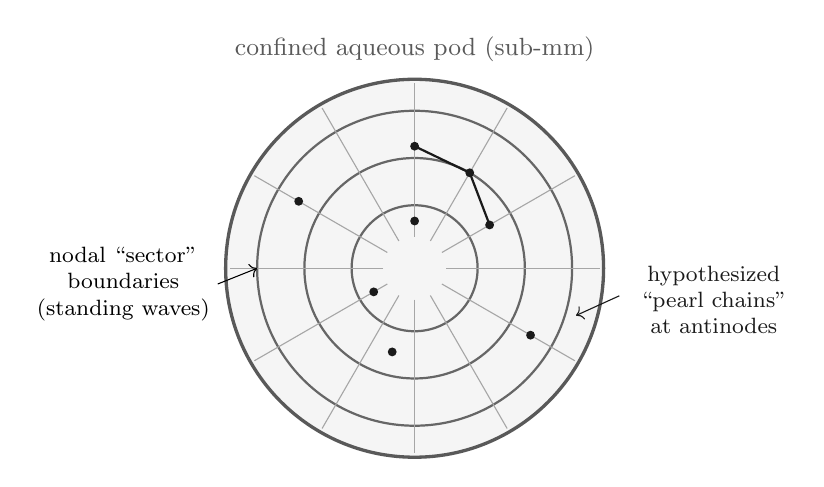
\begin{tikzpicture}[font=\small]
% pod boundary
\draw[acpcmteal,very thick,fill=acpcmteal!6] (0,0) circle (2.4cm);
\node[acpcmteal] at (0,2.78) {confined aqueous pod (sub-\unit{\milli\meter})};
% standing-wave nodal grid (concentric + radial = CHS analogy)
\foreach \r in {0.8,1.4,2.0} \draw[acpcmblue!60,thick] (0,0) circle (\r);
\foreach \a in {0,30,...,330} \draw[acpcmblue!35] (\a:0.4) -- (\a:2.35);
% a few "water pearls / chains" sitting at nodes
\foreach \pt in {(30:1.1),(150:1.7),(255:1.1),(330:1.7),(90:0.6),(210:0.6)}{
  \fill[warnrule] \pt circle (1.6pt);
}
\draw[warnrule,thick] (30:1.1) -- (60:1.4) -- (90:1.55);
\fill[warnrule] (60:1.4) circle (1.6pt);
\fill[warnrule] (90:1.55) circle (1.6pt);
% labels
\node[align=center,acpcmblue,font=\footnotesize] at (-3.7,-0.2)
  {nodal ``sector''\\boundaries\\(standing waves)};
\draw[->,acpcmblue,thin] (-2.5,-0.2) -- (-2.0,0.0);
\node[align=center,warnrule,font=\footnotesize] at (3.8,-0.4)
  {hypothesized\\``pearl chains''\\at antinodes};
\draw[->,warnrule,thin] (2.6,-0.35) -- (2.05,-0.6);
\end{tikzpicture}
\caption{Schematic of a pod with a cymatic cylinder--head--sector (CHS) analogue.
Concentric and radial standing-wave nodes (blue) partition the pod into addressable
voxels - the established, but transient, particle-patterning physics. The hypothesized
``pearl chains'' resident at antinodes (amber) belong to the contested structured-water
premise (\cref{as:cymgrid}). Not to scale.}
\label{fig:pod}
\end{figure}

%================================================================== 4. Write
\section{Encoding and writing: the ``broadcast-and-freeze'' mechanism}
\label{sec:write}

\subsection{Encoding by elemental sonification}
Digital payloads are mapped to acoustic spectra. \emph{Data sonification} - the principled
mapping of data to non-speech sound - is a mature methodology with an NSF-commissioned
status report~\cite{kramer1999nsf}, a canonical handbook~\cite{hermann2011handbook}, and a
formal taxonomy whose defining criterion is that the sound reflect \emph{objective}
properties of the data through a systematic, reproducible
transform~\cite{hermann2008taxonomy}. Mapping the wavelengths of atomic emission lines into
the audio band is a documented technique used for analysis, accessibility, and
education - e.g.\ the audification of astronomical spectra~\cite{trayford2023spectra} and
an interactive sonified periodic table~\cite{smith2024periodic}. ACPCM uses such a mapping
as a codebook: payload symbols index a dictionary of multi-tone acoustic ``words.'' These
audio-band tones serve as \emph{codebook symbols}, not literal drive frequencies: the
transducer operates in the MHz band (\cref{sec:format}), and each symbol indexes a distinct
multi-tone pattern within it.

It is essential to be precise about what sonification \emph{is not}. The light-to-audio
mapping (from ${\sim}10^{14}$\,Hz to ${\sim}10^{2}$--$10^{4}$\,Hz) is an arbitrary,
reproducible rescaling chosen for human perceptibility~\cite{smith2024periodic}; it is
\emph{not} a physical resonance, it reveals no ``hidden physics,'' and it carries no
information beyond what is already in the source data~\cite{hermann2008taxonomy}. The draft
framing additionally invokes W.~Russell's octave cosmology, in which the elements are
arranged on a spiral of ten octaves balancing ``centripetal'' and ``centrifugal''
tendencies~\cite{russell1926universalone}. We are explicit that this is a
\textbf{historical/esoteric} system - metaphysics, not chemistry - used here, if at all,
only as one arbitrary-but-fixed codebook among many. Nothing in the architecture depends on
Russell's metaphysics being correct; any injective, noise-separated frequency code would
serve, and a \emph{designed} code (e.g.\ orthogonal frequency-division multiplexing) is
strictly preferable.

\subsection{Writing by phase change}
The pod is held near its freezing point. The transducer simultaneously broadcasts (i)~the
cymatic formatting field of \cref{sec:format} and (ii)~the data tones. While the field is
held, the pod undergoes an \emph{instantaneous phase transition} to a solid. In analogy to
the melt--quench programming of chalcogenide phase-change
memory~\cite{wuttig2007pcm,raoux2010pcm} - and, more loosely, to HAMR's heat-and-quench
write cycle~\cite{kryder2008hamr} - in which a pulse melts a bit and rapid cooling freezes
it into a distinct solid phase, the rapid solidification is hypothesized to ``record'' the
instantaneous acoustic field as a frozen-in topology - displacements, density modulations,
and interface positions locked into the lattice.

\begin{assumption}[Faithful commit]\label{as:commit}
Freezing transfers the broadcast acoustic field into a static, readable lattice topology
with sufficient fidelity and reproducibility to be decoded, and the transition's own
dynamics (stochastic nucleation, latent-heat release, ${\sim}9\%$ volumetric expansion,
dendritic growth) do not destroy the encoded pattern.
\end{assumption}

\Cref{as:commit} is the architecture's load-bearing physical claim and its most likely
point of failure; we return to it in \cref{sec:limits}. We emphasize that the HAMR and PCM
citations establish only that \emph{their own} rapid-quench mechanisms work; they provide
\emph{no} evidence that an acoustic field can be recorded by freezing water. That bridge is
ours, and it is conjecture.

\subsection{What the freezing-under-sound literature actually says}
\label{sec:sono}
There \emph{is} an established body of work in which ultrasound applied during freezing
leaves a structural imprint in the resulting ice - \emph{sonocrystallization}, or
ultrasound-assisted freezing (UAF), studied extensively in food and pharmaceutical
processing~\cite{zhang2021uafmech,islam2014radish,delgado2017reviewcontrol}. Power
ultrasound demonstrably triggers ice nucleation in supercooled water, shortens freezing
time, and controls ice-crystal size and dendrite morphology. At first glance this is
encouragement for \cref{as:commit}: sound applied during a freeze \emph{does} change the
solid that results.

The mechanism, however, cuts the wrong way, and honesty requires stating it plainly. The
established coupling is \emph{cavitation}: the field nucleates and collapses gas/vapour
bubbles, and those bubbles - not the field's spatial pattern - seed the
ice~\cite{zhang2021uafmech,saclier2010bubbles}; collapsing bubbles further emit microjets
and shock waves that \emph{fragment} growing dendrites into secondary
nuclei~\cite{zhang2021uafmech}. This is spatially \emph{stochastic} (bubble sites are random)
and pattern-\emph{destroying} (fragmentation erases fine structure), the opposite of a
faithful field-to-lattice transcription. So the one real sound$\rightarrow$ice channel
supports the weak claim (a patterned freeze differs from a sham freeze) while actively
undermining the strong one ACPCM needs (the difference \emph{is} a readable copy of the
field). \Cref{sec:limits} draws the consequence: the cheapest test, \cref{pr:transfer}, is at
risk of a \emph{misleading positive} driven by cavitation rather than recording, and must be
designed to exclude it.

\subsection{A buildable special case: acoustically assembled, then locked}
\label{sec:assembly}
One variant of the write step is \emph{not} speculative at all, and we flag it as the
project's honest engineering exit. If the pod is seeded with discrete, acoustically
responsive tracer objects (micro-particles, beads, or cells), then arranging them at the
standing-wave nodes and \emph{locking} them in place by solidifying the surrounding medium
is demonstrated, current technology: holographic ultrasound fields assemble particles, gel
beads, and cells into prescribed 3D shapes that are then fixed permanently by gelation of the
host medium~\cite{melde2023assembly}, and acoustic focusing of beads/cells in a droplet
followed by cross-linking locks their positions to within ${\sim}10\%$ of the target
line~\cite{olofsson2021hydrogel}. Substitute ``freeze'' for ``gel'' and this is precisely
ACPCM's write--lock cycle, minus the speculative leap.

The price of buildability is that this records the \emph{positions of seeded objects}, not
the topology of the water itself - it is a particle-in-matrix memory, not ``molecular
cymatics.'' It still inherits the acoustic read limit of \cref{sec:diffraction} (the locked
pattern is read no finer than the ice wavelength), so it does not rescue the density verdict;
and it is a more modest claim than the pure-water proposal. We include it because it draws
the boundary exactly: everything up to and including \emph{assemble-and-lock discrete
scatterers} is established; the single remaining conjecture is that the same freeze records
the \emph{continuous water field} with no seeded objects at all (\cref{as:commit}).

%================================================================== 5. Read
\section{Reading: megahertz acoustic holography}
\label{sec:read}

Once committed to ice, the data lives in microscopic features of the solid, far below the
resolution of any microphone. Read-back is posed as an \emph{acoustic holography}
problem~\cite{melde2016holograms}.

\paragraph{The ice as a phase plate.}
A megahertz ultrasonic pulse illuminates the frozen pod. (That an acoustic probe can
interrogate the water-to-ice transition at all is established: MHz plate waves resolve the
freezing transition through its attenuation signature~\cite{anisimkin2021platewave}.)
Because acoustic holography is
diffraction-limited, resolving microscopic features requires correspondingly short
wavelengths - i.e.\ MHz (or higher) ultrasound, with millimetre-to-sub-millimetre
wavelengths in water and ice~\cite{melde2016holograms,jimenez2019skull}. The ice topology
then acts as a passive \emph{acoustic phase plate}~\cite{melde2016holograms,brown2019phaseamp}:
the scattered wave is transformed into a complex, three-dimensional volumetric pressure
field that encodes the structure it bounced off, and such plates can in principle be
stacked or reconfigured to multiplex fields~\cite{brown2020stackable}.

\paragraph{Capturing the field.}
The scattered field is sampled by a calibrated needle hydrophone over a measurement
surface, the standardized method for spatially mapping ultrasound
pressure~\cite{iec62127}. We note an honest caveat from the metrology literature: while
focal-pressure measurements can be highly \emph{repeatable} (coefficient of variation
below 2\%), inter-hydrophone \emph{agreement} for tightly focused MHz fields can differ by
tens of percent due to spatial averaging and frequency-response
uncertainty~\cite{martin2019hydrophone} - a real ceiling on read fidelity. A frequently
proposed enhancement is \emph{vectorial} sensing: recording not only the scalar pressure
$p$ but the particle-velocity components $(v_x,v_y)$. We flag, however, that in a fluid
these are \emph{not} independent degrees of freedom - they are fixed by spatial gradients
of the same scalar pressure via Euler's relation - so they add an information
\emph{dimension} under a physical constraint rather than free, independent bandwidth; this
remains an emerging idea, not a settled gain.

\paragraph{Neural decoding.}
Finally, the measured field is inverted to the original bitstream by a deep network - e.g.\
a U-Net of the kind already used for fast acoustic-hologram
synthesis~\cite{lin2021dlholograms}. The network \emph{architecture} is mature, but the
\emph{inverse} field-to-source decoding ACPCM requires is harder and less established than
the forward synthesis those works demonstrate: such inverse problems are ill-posed and a
network can hallucinate plausible outputs, so any demonstration must include held-out,
information-theoretic controls (\cref{pr:decode}).

%================================================================== read figure
\begin{figure}[t]
\centering
\resizebox{\textwidth}{!}{%
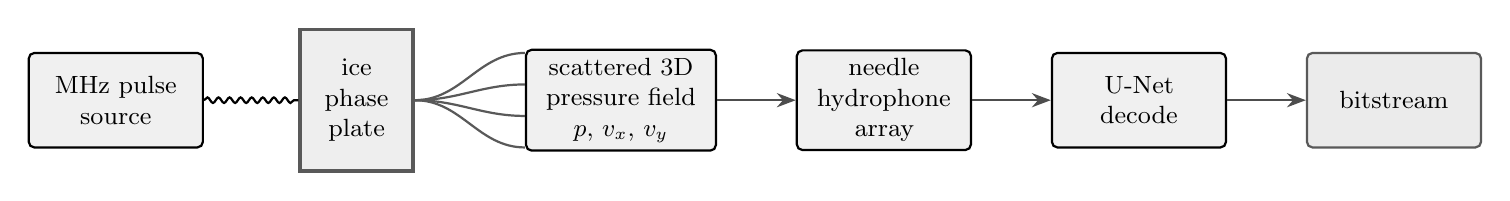
\begin{tikzpicture}[font=\small,node distance=10mm,
  blk/.style={draw=acpcmblue,thick,rounded corners=2pt,fill=acpcmblue!6,align=center,
    minimum height=12mm,text width=20mm,inner sep=3pt},
  arr/.style={-{Stealth[length=2.4mm]},acpcmgray,thick}]
% MHz source
\node[blk] (src) {MHz pulse\\source};
% ice phase plate
\node[draw=acpcmteal,very thick,fill=acpcmteal!10,minimum width=10mm,minimum height=18mm,
  right=12mm of src,align=center,text width=12mm] (plate) {ice\\phase\\plate};
% incoming wave
\draw[acpcmblue,thick,decorate,decoration={snake,amplitude=1pt,segment length=4pt}]
  (src.east) -- (plate.west);
% scattered 3D field
\node[blk,right=14mm of plate,text width=22mm] (field) {scattered 3D\\pressure field\\$p,\,v_x,\,v_y$};
\foreach \dy in {-6,-2,2,6}
  \draw[acpcmteal,thick] (plate.east) to[out=0,in=180]
    ($(field.west)+(0,\dy mm)$);
% hydrophone + unet
\node[blk,right=10mm of field] (hyd) {needle\\hydrophone\\array};
\node[blk,right=10mm of hyd] (unet) {U-Net\\decode};
\node[blk,right=10mm of unet,fill=acpcmteal!12,draw=acpcmteal] (bits) {bitstream};
\draw[arr] (field) -- (hyd);
\draw[arr] (hyd) -- (unet);
\draw[arr] (unet) -- (bits);
\end{tikzpicture}%
}
\caption{Read chain. A megahertz pulse scatters off the frozen pod, whose topology acts as
an acoustic phase plate~\cite{melde2016holograms}; the resulting volumetric field (scalar
pressure plus, optionally, particle-velocity components) is sampled by a hydrophone
array~\cite{iec62127,martin2019hydrophone} and inverted to a bitstream by a trained
network~\cite{lin2021dlholograms}. This read chain reuses only established techniques;
the speculative burden lies entirely on the write side (\cref{as:commit}).}
\label{fig:read}
\end{figure}

%================================================================== Capacity / density / energy
\section{Capacity, density, and energy: a quantitative reckoning}
\label{sec:capacity}

An architecture proposal that omits the numbers is untestable as engineering. Here we put
ACPCM on the same axes as real storage. The conclusion is unflattering and, we think,
clarifying: the binding limit is not how finely water can be arranged but the wavelength of
the wave used to read it, and on that limit ACPCM is many orders of magnitude short of every
incumbent.

\subsection{The optimistic ceilings (granted, then discounted)}
A \qty{1}{\micro\liter} pod (a \qty{1}{\milli\meter} cube of water, ${\sim}\qty{1}{\milli\gram}$)
holds ${\sim}3.3\times10^{19}$ molecules. A naive ``one bit per molecule'' bound therefore
suggests ${\sim}3\times10^{19}$ bits ($\approx$ 4\,EB) \emph{per microlitre} - a physically
meaningless upper bound, but a useful ceiling.

The structured-water literature supplies a more specific, internally quantified claim, which
we state explicitly and \emph{without endorsement} (it rests on the contested ``fourth-phase''
premise~\cite{pollack2013fourth,elton2020ez}). In that account the storage unit is not a
molecule but a ${\sim}\qty{15}{\nano\meter}$ ``pearl'' of ${\sim}85{,}000$ molecules; pearls
link into ${\sim}\qty{300}{\nano\meter}$ ``chains'' of ${\sim}20$ pearls, with chains below
${\sim}\qty{100}{\nano\meter}$ deemed too short to resolve a distinct signature. Treating one
chain (a ${\sim}\qty{15}{\nano\meter}$-wide, ${\sim}\qty{300}{\nano\meter}$-long cylinder,
${\sim}5.3\times10^{4}\,\mathrm{nm}^3$) as one symbol gives ${\sim}1.9\times10^{16}$
chains/cm$^3$, i.e.\ the literature's own headline of ${\sim}1.9\times10^{16}$ bytes/cm$^3$
($\approx$ 19\,TB per microlitre, ${\sim}700\times$ the density of 5D
glass)~\cite{pollack2013fourth}. We carry this figure forward only to show, next, that even
granting it in full changes nothing: a constraint downstream of storage dominates.

\subsection{The diffraction limit sets the real ceiling}
\label{sec:diffraction}
Read-out is acoustic (\cref{sec:read}) and - crucially - propagates through the frozen
\emph{ice}, where the sound speed is $c\approx\qty{3200}{\meter\per\second}$, roughly twice
the $\qty{1500}{\meter\per\second}$ of liquid water. Spatial resolution is bounded by the
probe wavelength \emph{in that medium}: a \qty{50}{\mega\hertz} read pulse has
$\lambda\approx\qty{64}{\micro\meter}$ in ice and resolves voxels no finer than
$\lambda/2\approx\qty{32}{\micro\meter}$. (Features may be \emph{written} more finely - the
cymatic field forms in the liquid, where $\lambda/2\approx\qty{15}{\micro\meter}$ - but they
cannot be \emph{read} below the ice limit, so the channel is read-limited.) Absorption climbs
as ${\sim}f^2$, so halving the voxel by going to ${\sim}\qty{100}{\mega\hertz}$ costs steeply
in penetration depth - a hard, physics-imposed resolution--penetration trade. A
\qty{1}{\milli\meter} pod thus contains ${\sim}(1000/32)^3\approx 3\times10^{4}$ resolvable
voxels; allotting several bits per voxel by exploiting phase and amplitude lifts this only to
${\sim}10^{5}$ bits - of order \qty{10}{\kilo\byte} per cubic-millimetre pod.\footnote{The
two-axis scheme of \cref{sec:biaxial} makes the budget concrete and, deliberately, more
conservative: a \qty{5}{\mega\hertz} axial former (liquid-phase
$\lambda_z\approx\qty{300}{\micro\meter}$) writes ${\sim}6$ coarse, freeze-robust discs
across a \qty{1}{\milli\meter} pod - well above the ice read limit, so all are resolvable -
while the read-limited transverse cells number ${\sim}(1000/32)^2\approx 10^{3}$ per disc,
for ${\sim}6\times10^{3}$ voxels: below the isotropic ${\sim}3\times10^{4}$ ceiling, the
price of trading resolution for a coarse, freeze-robust layer index.}

The verdict follows immediately. The realistic ${\sim}10^{5}$ bits/mm$^3$ sits roughly
\emph{nine} orders of magnitude below the structured-water theory's own
${\sim}1.5\times10^{14}$ bits/mm$^3$, and roughly \emph{fourteen} below the
one-bit-per-molecule ceiling. \emph{You cannot read what you cannot resolve}; the molecular
real estate is irrelevant if the only available probe paints it with a
${\sim}\qty{32}{\micro\meter}$ brush.
This is the quantitative core of why ACPCM, even with every contested premise granted, is not
a high-density medium.

\begin{figure}[t]
\centering
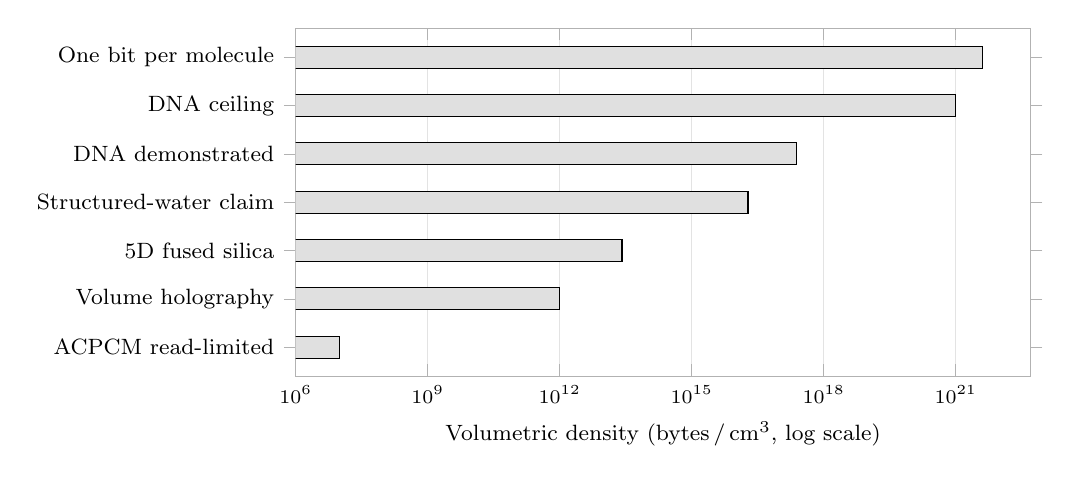
\begin{tikzpicture}
\begin{axis}[
  xmode=log, xmin=1e6, xmax=5e22,
  width=0.9\textwidth, height=6cm,
  xbar, bar width=8pt,
  xlabel={Volumetric density (bytes\,/\,cm$^3$, log scale)},
  xlabel style={font=\footnotesize},
  symbolic y coords={ACPCM read-limited,Volume holography,5D fused silica,Structured-water claim,DNA demonstrated,DNA ceiling,One bit per molecule},
  ytick=data,
  yticklabel style={font=\footnotesize},
  xtick={1e6,1e9,1e12,1e15,1e18,1e21},
  xticklabel style={font=\scriptsize},
  enlarge y limits=0.10,
  axis line style={gray!60}, tick style={gray!60},
  xmajorgrids, grid style={gray!22,thin},
]
\addplot[draw=black, fill=black!12] coordinates {
  (1e7,ACPCM read-limited)
  (1e12,Volume holography)
  (2.6e13,5D fused silica)
  (1.9e16,Structured-water claim)
  (2.4e17,DNA demonstrated)
  (1e21,DNA ceiling)
  (4e21,One bit per molecule)};
\end{axis}
\end{tikzpicture}
\caption{Volumetric storage density across media (log scale; figures as in \cref{tab:comparators}).
The read-limited ACPCM reality (bottom, this work) sits roughly nine orders of magnitude below the
structured-water theory's own claim and fourteen below the one-bit-per-molecule ceiling, and below
every established medium. The binding constraint is the ice-borne read wavelength
(\cref{sec:diffraction}), not how finely matter can be arranged.}
\label{fig:density}
\end{figure}

\subsection{Energy and throughput}
Committing a bit means freezing a droplet. Removing heat from a pod of mass $m$ held
$\Delta T$ above freezing costs at least $E = m\,(c_p\,\Delta T + L_{\mathrm{f}})$, with
$c_p\approx\qty{4.18}{\joule\per\gram\per\kelvin}$~\cite{iapws95} and
$L_{\mathrm{f}}\approx\qty{333.5}{\joule\per\gram}$~\cite{osborne1939fusion}. For a
\qty{1}{\micro\liter} pod cooled \qty{20}{\kelvin} then frozen,
$E\approx\qty{1e-3}{\gram}\times(84+333.5)\,\unit{\joule\per\gram}\approx\qty{0.42}{\joule}$.
Spread over the diffraction-limited ${\sim}10^{5}$ bits, that is ${\sim}\qty{4e-6}{\joule}$
per bit (${\sim}4\,\mu$J/bit) of heat that must be \emph{removed} - by a refrigerator with
coefficient of performance well below unity, multiplying the wall-plug cost several-fold,
and before counting transducer drive, hydrophone scan, and neural inversion. Incumbent
operations sit at the picojoule-per-bit scale (on-chip and DRAM access; 3D-NAND programming
amortizes to ${\sim}$\,pJ--tens-of-pJ per bit)~\cite{horowitz2014energy}. ACPCM's write
energy is therefore ${\sim}10^{5}$--$10^{7}\times$ worse per bit before refrigeration
overhead. Throughput compounds it: freezing is a stochastic-nucleation event on
millisecond-and-slower scales against HAMR's sub-nanosecond per-bit write~\cite{kryder2008hamr},
and because rewriting demands re-melting, the medium is closer to write-once archival than to
random-access memory.

\begin{figure}[t]
\centering
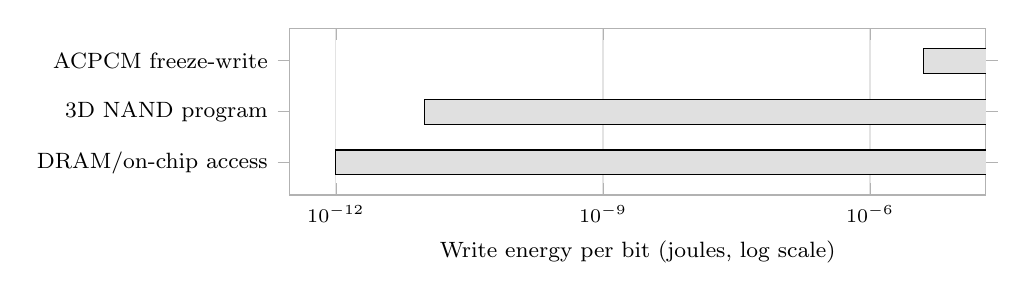
\begin{tikzpicture}
\begin{axis}[
  xmode=log, xmin=3e-13, xmax=2e-5,
  width=0.86\textwidth, height=3.7cm,
  xbar, bar width=9pt,
  xlabel={Write energy per bit (joules, log scale)},
  xlabel style={font=\footnotesize},
  symbolic y coords={DRAM/on-chip access,3D NAND program,ACPCM freeze-write},
  ytick=data, yticklabel style={font=\footnotesize},
  xtick={1e-12,1e-9,1e-6}, xticklabel style={font=\scriptsize},
  enlarge y limits=0.32,
  axis line style={gray!60}, tick style={gray!60},
  xmajorgrids, grid style={gray!22,thin},
]
\addplot[draw=black, fill=black!12] coordinates {
  (1e-12,DRAM/on-chip access)
  (1e-11,3D NAND program)
  (4e-6,ACPCM freeze-write)};
\end{axis}
\end{tikzpicture}
\caption{Write energy per bit (log scale). Freezing a ${\sim}\qty{1}{\micro\liter}$ pod and
amortizing over its ${\sim}10^{5}$ read-limited bits costs ${\sim}\qty{4}{\micro\joule}$ of heat
removed per bit (\cref{sec:capacity}) - five to seven orders of magnitude above incumbent
picojoule-scale operations~\cite{horowitz2014energy}, and that is before refrigeration overhead,
transducer drive, and neural decoding.}
\label{fig:energy}
\end{figure}

\begin{table}[t]
\centering
\small
\renewcommand{\arraystretch}{1.25}
\begin{tabularx}{\textwidth}{@{}>{\raggedright\arraybackslash}p{0.27\textwidth}
  >{\raggedright\arraybackslash}p{0.30\textwidth}
  >{\raggedright\arraybackslash}X@{}}
\toprule
\textbf{Medium} & \textbf{Volumetric density (order)} & \textbf{Status / note} \\
\midrule
5D fused-silica glass
  & ${\sim}26$\,TB/cm$^3$
  & \textcolor{acpcmteal}{\bfseries Emerging}; ${\sim}10^{20}$-yr decay, \qty{1000}{\celsius} stable~\cite{zhang2014glass,lei2021optica} \\
DNA (synthesized oligos)
  & ${\sim}215$\,PB/g (${\sim}10^{17}$\,B/cm$^3$); ceiling ${\sim}10^{18}$\,B/mm$^3$
  & \textcolor{acpcmteal}{\bfseries Emerging}; random access demonstrated~\cite{erlich2017fountain,ceze2019molecular} \\
Volume holography
  & ${\sim}1/\lambda^3$ (order $1$\,TB/cm$^3$)
  & \textcolor{acpcmgray}{\bfseries Niche}; theoretical bound~\cite{heanue1994holographic,coufal2000holographic} \\
ACPCM - structured-water accounting
  & ${\sim}1.9\times10^{16}$\,B/cm$^3$ (19\,TB/$\mu$L)
  & \textcolor{warnrule}{\bfseries Speculative}; contested premise~\cite{pollack2013fourth} \\
ACPCM - diffraction-limited reality
  & ${\sim}10^{7}$\,B/cm$^3$ (${\sim}10^{5}$ bits/mm$^3$)
  & \textbf{This work}; set by ice read wavelength (\cref{sec:diffraction}) \\
\bottomrule
\end{tabularx}
\caption{ACPCM against unconventional storage media on volumetric density. DNA per-cm$^3$
assumes a dry density ${\sim}\qty{1.1}{\gram\per\centi\meter\cubed}$. The two ACPCM rows bracket the
gap between what the contested premise claims and what the acoustic read path can actually
resolve: ${\sim}9$ orders of magnitude, with a further ${\sim}5$ to the one-bit-per-molecule
ceiling. The realistic ACPCM density is below every established medium in the table.}
\label{tab:comparators}
\end{table}

%================================================================== Epistemic ledger
\section{Epistemic ledger}
\label{sec:ledger}

\Cref{tab:status} is the paper's central honesty device: each subsystem is paired with the
real-world mechanism it borrows and with a blunt status label. The pattern is deliberate:
\emph{the read path and the write \textbf{actuation} are built from established techniques,
while the speculative weight is concentrated in a small number of clearly marked assumptions
about how freezing water records and preserves an acoustic field.} The refuted ingredient
(``water memory'') is load-bearing nowhere; it is motivational framing only.

\begin{table}[!t]
\centering
\small
\renewcommand{\arraystretch}{1.25}
\begin{tabularx}{\textwidth}{@{}>{\raggedright\arraybackslash}p{0.21\textwidth}
  >{\raggedright\arraybackslash}X
  >{\raggedright\arraybackslash}p{0.205\textwidth}@{}}
\toprule
\textbf{ACPCM subsystem} & \textbf{Borrowed real mechanism} & \textbf{Status of the leap} \\
\midrule
Rapid ``write'' by phase change (\cref{sec:write})
  & HAMR heat--quench; chalcogenide PCM melt--quench switching~\cite{kryder2008hamr,wuttig2007pcm}
  & \textcolor{warnrule}{\bfseries Speculative} (\cref{as:commit}) \\
Assemble-and-lock seeded scatterers (\cref{sec:assembly})
  & Holographic acoustic assembly fixed by gelation; acoustic focusing $+$ cross-link~\cite{melde2023assembly,olofsson2021hydrogel}
  & \textcolor{acpcmteal}{\bfseries Established} for \emph{particles}; the leap is pure-water recording \\
Sound$\rightarrow$ice structural imprint (\cref{sec:sono})
  & Sonocrystallization / ultrasound-assisted freezing~\cite{zhang2021uafmech,delgado2017reviewcontrol}
  & Imprint \textcolor{acpcmteal}{\bfseries established} but via \textcolor{warnrule}{\bfseries cavitation} (stochastic, pattern-destroying) \\
Ordered ice by directional freeze (\cref{sec:device})
  & Freeze-casting; planar-front stability; magnetic grain alignment~\cite{deville2006freezecast,mullins1964stability,porter2012magnetic}
  & \textcolor{acpcmteal}{\bfseries Established} at scale; the device regime, not the chaotic quench \\
Cell isolation via pods (\cref{sec:medium})
  & Charge-trap flash discrete traps~\cite{white2000sonos}
  & \textcolor{acpcmgray}{\bfseries Plausible} (\cref{as:confine}) \\
Cymatic addressing grid (\cref{sec:format})
  & Acoustofluidic patterning; holographic tweezers~\cite{rufo2022acoustofluidics,marzo2015holographic}
  & Particle nodes \textcolor{acpcmteal}{\bfseries established}; molecular ordering \textcolor{warnrule}{\bfseries speculative} (\cref{as:cymgrid}) \\
Two-axis disc addressing (\cref{sec:biaxial})
  & Drive track/sector split; axial vs.\ transverse standing waves
  & Geometry \textcolor{acpcmgray}{\bfseries plausible}; survival through freeze \textcolor{warnrule}{\bfseries speculative} (\cref{as:biaxial}) \\
Sonification codebook (\cref{sec:write})
  & Data-sonification methodology~\cite{kramer1999nsf,hermann2011handbook}
  & Mapping \textcolor{acpcmteal}{\bfseries established}; Russell octaves \textcolor{warnrule}{\bfseries esoteric/optional}~\cite{russell1926universalone} \\
MHz acoustic-holography read-out (\cref{sec:read})
  & Acoustic holograms; hydrophone metrology; DL inversion~\cite{melde2016holograms,martin2019hydrophone,lin2021dlholograms}
  & \textcolor{acpcmteal}{\bfseries Established} techniques \\
``Structured-water'' carriers (\cref{sec:medium})
  & EZ/fourth-phase water; Orch-OR water~\cite{pollack2013fourth,hameroff2014orchor}
  & \textcolor{warnrule}{\bfseries Contested / minority}~\cite{elton2020ez,tegmark2000decoherence} \\
``Water memory'' (motivation only)
  & Benveniste high-dilution claims~\cite{benveniste1988}
  & \textbf{Refuted}~\cite{maddox1988} \\
\bottomrule
\end{tabularx}
\caption{Epistemic ledger mapping each ACPCM subsystem to its borrowed real mechanism and
the status of the conceptual leap. The architecture is engineered so that the
\emph{refuted} ingredient (water memory) carries \emph{no} load - it is motivational
framing only - while the genuinely novel risk is isolated in \cref{as:commit}. Established
citations support only their own row and lend no credibility to the speculative rows.}
\label{tab:status}
\end{table}

%================================================================== 7. Predictions
\section{Falsifiable predictions}
\label{sec:predictions}

A speculative proposal earns its keep by being testable. ACPCM implies concrete, disprovable
predictions; any one of them failing falsifies the corresponding assumption.

\begin{prediction}[Field-to-lattice transfer]\label{pr:transfer}
Freezing a thin water film while broadcasting a fixed MHz pressure pattern produces a
\emph{reproducible}, pattern-dependent modulation in the resulting ice (e.g.\ in density,
birefringence, or scattered-field signature) that is absent under sham (unmodulated)
freezing. \emph{Test:} interferometric or acoustic readout of patterned vs.\ control
freezes under blinding; \emph{falsified if} no above-noise, pattern-correlated structure
survives (\cref{as:commit}).

\emph{Mandatory confound control.} A bare positive here is \textbf{not} sufficient, because
sonocrystallization guarantees that \emph{any} insonated freeze differs from a quiescent one
through cavitation-seeded nucleation and dendrite fragmentation
(\cref{sec:sono})~\cite{zhang2021uafmech} - an effect that carries no field information. The
test must therefore (i)~suppress cavitation as a confound (degassed water, elevated static
pressure, or amplitudes below the cavitation threshold), and (ii)~demand that the imprint
\emph{tracks the imposed pattern's geometry} - changing with node spacing and orientation and
registering to the antinode lattice - rather than merely exceeding the sham. A difference
that does not move with the pattern is a cavitation artefact, not a recording, and counts as a
\emph{falsification}, not a success.
\end{prediction}

\begin{prediction}[Addressable nodes]\label{pr:nodes}
The post-freeze structure is spatially organized at the wavelength scale of the imposed
standing wave. \emph{Falsified if} the frozen modulation shows no correlation with the node
geometry (\cref{as:cymgrid}).
\end{prediction}

\begin{prediction}[Decodable channel]\label{pr:decode}
A network trained on (pattern $\rightarrow$ scattered-field) pairs recovers the input code
above chance on held-out patterns, with a measurable channel capacity. \emph{Falsified if}
decoding accuracy is at chance on held-out data, indicating no recoverable information (and
guarding against the network merely memorizing or hallucinating).
\end{prediction}

\begin{prediction}[Diffraction-bounded, two-axis capacity]\label{pr:capacity}
The recoverable channel capacity per pod scales as ${\sim}(D/\lambda)^3$ in the pod diameter
$D$ and read wavelength $\lambda$, and a low-frequency axial former produces a separable
layer index (\cref{as:biaxial}): the decoder recovers \emph{which disc} a feature occupies
independently of the in-disc payload. \emph{Falsified if} the layer index is not separable,
\emph{or} - the genuinely exciting failure - if recovered capacity \emph{exceeds} the
acoustic diffraction ceiling of \cref{sec:diffraction}, which would imply a sub-wavelength
read channel and overturn the pessimistic density verdict.
\end{prediction}

If \cref{pr:transfer} fails - the most likely outcome given current physics - the
architecture collapses to its established components, and that negative result is itself
worth reporting.

%================================================================== 8. Limitations
\section{Discussion: obstacles, limits, and why this is hard}
\label{sec:limits}

We do not claim ACPCM is feasible. The honest reading is that it is \emph{probably not},
for reasons worth stating precisely because they sharpen the predictions above.

\paragraph{The freezing transition is violent.}
On freezing, water releases its latent heat of fusion, $L_{\mathrm{f}}\approx\qty{333.5}{\joule\per\gram}$~\cite{osborne1939fusion},
and expands by ${\sim}9\%$ as it drops from ${\sim}\qty{1.0}{\gram\per\centi\meter\cubed}$ to
the ${\sim}\qty{0.917}{\gram\per\centi\meter\cubed}$ of hexagonal ice
$\mathrm{I_h}$~\cite{iapws95}; nucleation is stochastic and growth is dendritic. Any acoustic
``imprint'' must survive this disordering, mechanically disruptive event. A ${\sim}9\%$
volume change (a ${\sim}3\%$ linear strain) at a voxel scale of
$\lambda/2 \approx 15$--$75\,\unit{\micro\meter}$ (10--50\,MHz in water) implies linear
displacements of order ${\sim}0.5$--$2\,\unit{\micro\meter}$ - a non-negligible fraction of
the intended nodal spacing itself, directly threatening the registration the two-axis scheme
depends on (\cref{as:biaxial,as:commit}).

\emph{The obvious escape - vitrify rather than crystallize - is itself punishing.} Forming
amorphous (glassy) ice instead of dendritic $\mathrm{I_h}$ avoids the worst of the
crystallization disruption, but pure water vitrifies only above a critical cooling rate
recently measured at ${\sim}6.4\times10^{6}\,\unit{\kelvin\per\second}$~\cite{schmidt2025cooling}
(first demonstrated by hyperquenching micron-scale droplets~\cite{bruggeller1980vitrification}),
practical only for very small volumes - in direct tension with the ${\sim}\qty{15}{\micro\meter}$
voxels the read path can resolve (\cref{sec:diffraction}). Crystallize instead and you race a
moving front: dendritic ice tip velocities reach ${\sim}0.1$--$10\,\unit{\centi\meter\per\second}$
at moderate supercooling~\cite{shibkov2003ice,xu2016ice}, fast enough to sweep a
${\sim}\qty{15}{\micro\meter}$ voxel in microseconds and rearrange whatever the field had
arranged. Homogeneous nucleation does not even begin until the classical limit of
${\sim}\qty{235}{\kelvin}$ (${\sim}\qty{-38}{\celsius}$), so the ``hold the field, then
freeze'' write cycle must thread a narrow window of deep supercooling. \Cref{as:commit} is thus in
direct tension with the thermodynamics of solidification on every axis - rate, habit, and
strain - and controlling nucleation site, rate, and crystal habit ($\mathrm{I_h}$ vs.\
vitrified) is a hard, partly unsolved problem in its own right.

\paragraph{The only established sound$\rightarrow$ice channel is the wrong one.}
It would be convenient if the sonocrystallization literature
(\cref{sec:sono})~\cite{zhang2021uafmech,delgado2017reviewcontrol} supplied the missing
mechanism. It does not. That literature couples sound to ice through \emph{cavitation} -
bubble nucleation and collapse - which seeds ice at \emph{stochastic} sites and fragments
dendrites~\cite{zhang2021uafmech,saclier2010bubbles}; it changes ice statistics, not ice
\emph{coordinates}. A faithful commit (\cref{as:commit}) needs the inverse: a deterministic,
spatially registered transcription of a continuous field. The established effect is thus
simultaneously the best evidence that freezing-under-sound does \emph{something} and the
clearest reason to expect that something to be informationally empty - which is exactly why
\cref{pr:transfer} carries a mandatory cavitation control.

\paragraph{What the nearest experiments actually show.}
No one has performed the exact ACPCM experiment - impose a cymatic standing wave in bulk
water, freeze, and recover spatial information - but the closest containerless-freezing work
is consistent on the point that matters. When a water droplet is frozen while held in an
acoustic levitation field, it supercools, nucleates a crust, and then solidifies by
\emph{inward dendritic growth}; the field's role is to \emph{hold} the droplet without a
container, not to write its interior, and the resulting ice records the thermal field and
crystallography, not the acoustic node geometry~\cite{biswas2025snowflake}. Where an imposed
field \emph{does} leave a preserved pattern, it does so by arranging \emph{discrete objects}:
suspended particles in a levitated or drying droplet are driven to the pressure field's nodes
and that arrangement survives into the dried/solid granule~\cite{yarin2002drying}. Both
observations reproduce the boundary of \cref{sec:assembly}: fields move and freeze
\emph{things}; ordinary crystallization writes the \emph{ice}.

\paragraph{Field-stabilised (containerless) freezing: a better rig, not a better device.}
A natural instinct is to hold each pod still and freeze it in place by a static field rather
than against a wall. This is real and worth using. Water is diamagnetic and can be
\emph{levitated} in a strong gradient magnetic field - the route by which Tagami and
co-workers performed containerless solidification of magnetically levitated water in a hybrid
magnet~\cite{tagami1999maglev}, and which a recent design achieves for ${\sim}\qty{0.3}{\milli\meter}$
droplets with only ordinary permanent magnets~\cite{naito2024diamaglev}; charged droplets are
likewise held contact-free in electrostatic levitators, the standard tool for
deep-undercooling solidification studies~\cite{rhim1993esl}. Static and oscillating magnetic
fields also demonstrably bias ice nucleation and crystal size~\cite{otero2016magnetic}, and the magnetic
anisotropy of ice even lets a strong field orient the crystal $c$-axis - a genuine lever on
habit and registration. The honest verdict is that this improves the \emph{experiment} rather
than the architecture: containerless levitation removes wall (heterogeneous) nucleation,
enables the deep, controlled supercooling \cref{as:commit} needs, and is in fact the cleanest
rig in which to run \cref{pr:transfer}. But it does not address the load-bearing failure - the
freeze front still overruns the pattern (above), the read path is still diffraction-limited
(\cref{sec:diffraction}), and a tesla-scale magnet or kilovolt trap \emph{per pod} runs
directly against the cheap-archival premise that motivates the medium. Levitation makes the
test honest; it does not make the device feasible.

\paragraph{Liquid water has no long-term memory.}
The hydrogen-bond network reorganizes on picosecond timescales~\cite{cowan2005water}; there
is no credible evidence for persistent information storage in \emph{liquid} water, and the
specific ``water memory'' claims invoked as motivation were investigated and not
reproduced~\cite{maddox1988,benveniste1988}, including later
revivals~\cite{montagnier2009}. ACPCM only sidesteps this objection by storing nothing in
the liquid - which places the entire burden on the freeze step.

\paragraph{Resolution versus penetration.}
Resolving microscopic features acoustically requires very high frequencies, where absorption
in water and ice rises steeply; there is a real, physics-imposed tension between resolution
and penetration that caps achievable density. Read-out is also an ill-posed inverse problem,
and hydrophone metrology already shows tens-of-percent inter-device disagreement for tightly
focused MHz fields~\cite{martin2019hydrophone}, so any demonstration must include rigorous,
blinded, information-theoretic controls (\cref{pr:decode}).

\paragraph{Thermodynamic and energy cost.}
Writing a bit by freezing and reading it by illumination implies an energy budget per bit
that is plausibly orders of magnitude worse than incumbent technologies, before considering
throughput. Even if every assumption held, the density/energy/latency envelope would need to
beat HAMR~\cite{kryder2008hamr} and 3D NAND~\cite{goda2020} to matter - a very high bar.

\paragraph{What would change our mind.}
A positive, replicated result on \cref{pr:transfer} under blinded controls \emph{with
cavitation excluded} - pattern-dependent, above-noise, geometry-tracking structure that
survives freezing and carries recoverable information - would promote \cref{as:commit} from
speculation to phenomenon and justify pursuing the rest. Absent that, the honest fallback is
not nothing: the particle-seeded, assemble-and-lock variant of \cref{sec:assembly} is already
demonstrated in adjacent fields~\cite{melde2023assembly,olofsson2021hydrogel} and is the
buildable core that survives if the pure-water conjecture fails. What dies in that case is
specifically the claim that water records a continuous acoustic field without seeded
scatterers; what remains is a modest, read-limited particle-in-ice memory and an organizing
metaphor for cross-disciplinary analogy, not a competitive storage technology.

%================================================================== Toward a device
\section{Toward a device that could stand}
\label{sec:device}

The preceding sections refute ACPCM as a \emph{high-density} memory. They do not, by
themselves, refute it as a \emph{device} - provided it stops competing on the axis it loses
and is rebuilt from the regimes where freezing water is \emph{controllable} rather than
chaotic. This section sketches that pivot in the same honest spirit as the rest of the paper:
it remains speculative, but it is now device-\emph{shaped} - a build recipe assembled from
individually demonstrated components, a concrete operating point, and a fresh set of
falsifiable tests. The key realization is that \emph{directional} solidification of water is
not a thought experiment but an industry: \emph{freeze-casting} (ice-templating) routinely
produces ordered, regular, repeatable ice architecture by controlling a freezing
front~\cite{deville2006freezecast}. ``Freezing is too chaotic to record structure'' is false
in that regime; it is true only of the uncontrolled, deeply supercooled quench assumed in
\cref{sec:limits}.

\subsection{Reframe the competition}
ACPCM should not be pitched on density or energy, where it loses to DNA, 5D glass, and DRAM
by the margins of \cref{sec:capacity}. It should be pitched on the axes where water is without
peer: \emph{substrate cost, abundance, non-toxicity, and recyclability}, deployed where cold
is already free. Water is the cheapest write medium on Earth; it requires no synthesis (unlike
DNA), is benign at any scale (unlike essentially every engineered medium), and is - uniquely -
\emph{infinitely re-writable at the substrate level}: melt it and the medium is pristine
again. The target is the coldest, cheapest, most disposable tier of the storage hierarchy -
the gravel of data storage, not the diamond.

\subsection{Four moves that turn each obstacle into a design choice}
Each load-bearing objection of \cref{sec:limits} maps to an established mechanism that
neutralizes it, at the cost of abandoning the pure-water, high-density framing.

\begin{enumerate}[leftmargin=1.6em,nosep]
  \item \textbf{Faithful commit $\rightarrow$ seed the scatterers.} Do not ask bare water to
  record the field. Seed the pod with acoustically responsive tracers and lock their
  field-assembled positions by freezing - the assemble-and-lock cycle already demonstrated
  with gelation~\cite{melde2023assembly,olofsson2021hydrogel} (\cref{sec:assembly}). This
  retires \cref{as:commit} entirely; the recorded quantity is particle position, which
  \emph{is} preserved through solidification.
  \item \textbf{Dendritic overrun $\rightarrow$ stay below the instability.} The freeze front
  destroys fine structure only \emph{above} the Mullins--Sekerka critical
  velocity~\cite{mullins1964stability}: below it, in a sufficiently steep thermal gradient,
  the solid--liquid interface is morphologically \emph{stable} and advances as a planar (or
  regularly cellular) front. Freeze-casting exploits exactly this to template ordered
  lamellae~\cite{deville2006freezecast}. Trade write speed for fidelity and the
  ``front overruns the pattern'' objection becomes a regime boundary to engineer around, not
  a law.
  \item \textbf{No addressable grid $\rightarrow$ encode in the grain architecture.} Let the
  directional freeze itself carry the data: lamellar spacing, the grain-boundary map, and -
  the multi-level axis - the crystallographic $c$-axis orientation of each grain, steered by a
  \emph{weak} (millitesla, not tesla) rotating magnetic bias during freezing, as in magnetic
  freeze-casting~\cite{porter2012magnetic}. Orientation read by acoustic (or birefringence)
  anisotropy gives more than one bit per grain. The mechanism that
  \cref{sec:limits} called a confound - fields steering nucleation and growth - becomes the
  \emph{signal}.
  \item \textbf{Energy/throughput $\rightarrow$ co-opt ambient cold.} The ${\sim}\qty{4}{\micro\joule}$/bit
  freeze cost (\cref{sec:capacity}) is a cost only where heat must be actively pumped. Site
  the medium where cold is free and standing - polar archives, the cold aisle of a cryogenic
  data centre, or lunar permanently-shadowed regions at ${\sim}\qty{40}{\kelvin}$ - and the
  budget collapses toward the transducer and read electronics. Re-melt-to-rewrite, a drawback
  for RAM, is reframed as built-in secure erasure plus substrate recycling.
\end{enumerate}

\subsection{The honest operating point}
This device is still acoustic-read-limited (\cref{sec:diffraction}): ${\sim}10^{4}$--$10^{7}$
bits/mm$^3$, below every incumbent on volumetric density, and energy-competitive only where
cold is ambient. We claim no density win and no energy win. The claim is narrower and, we
think, defensible: a \emph{non-empty niche} for an ultra-low-cost, non-toxic, substrate-recyclable,
geologically stable cold-archive tier, built from components each demonstrated in isolation.
Whether that niche is worth occupying is an economic question; that it is physically
constructible to test is the point.

\subsection{Device-mode predictions}
The pivot earns its keep only if it, too, is falsifiable. It adds three tests to those of
\cref{sec:predictions}.
\begin{prediction}[Planar-front fidelity]\label{pr:planar}
Recording fidelity of a seeded pattern is high when the front advances \emph{below} the
Mullins--Sekerka critical velocity~\cite{mullins1964stability} and degrades sharply above it.
\emph{Falsified if} fidelity is independent of front velocity (which would mean the imprint is
not a solidification-front effect at all).
\end{prediction}
\begin{prediction}[Recyclability]\label{pr:recycle}
The pod survives many melt--refreeze--rewrite cycles with no accumulating error floor.
\emph{Falsified if} dissolved-gas or solute build-up degrades readback within a few cycles -
the failure mode that would make ``infinitely re-writable'' false in practice.
\end{prediction}
\begin{prediction}[Orientation multi-level]\label{pr:orient}
A millitesla rotating bias during directional freezing sets per-grain $c$-axis orientation
that survives the full freeze and is recoverable by acoustic anisotropy, yielding
$>1$~bit/grain~\cite{porter2012magnetic}. \emph{Falsified if} orientation does not survive
solidification or cannot be read above chance.
\end{prediction}

Every block invoked here - acoustic assembly~\cite{melde2023assembly}, planar-front
directional solidification~\cite{mullins1964stability,deville2006freezecast}, magnetic grain
alignment~\cite{porter2012magnetic}, and acoustic-anisotropy read-out~\cite{anisimkin2021platewave} -
is established in isolation. The remaining conjecture is only that they \emph{compose} into a
working channel. That is the precise difference between a metaphor and a device, and it is a
conjecture one can build a bench to test.

\FloatBarrier % flush any remaining floats before the conclusion / references

%================================================================== 9. Conclusion
\section{Conclusion}
\label{sec:conclusion}

We have presented Acousto-Cymatic Phase-Change Memory as a structured thought experiment that
transposes two proven storage principles - rapid phase-change writing
(HAMR~\cite{kryder2008hamr}, PCM~\cite{wuttig2007pcm}) and microscopic isolation
(CTF~\cite{white2000sonos}) - onto a rapidly frozen aqueous medium, with an
acoustic-holographic, neural-decoded read path that reuses otherwise-established
techniques~\cite{melde2016holograms,lin2021dlholograms}. Its value is not a feasibility
claim but the discipline of the synthesis: by laying out an explicit epistemic ledger
(\cref{tab:status}) and a falsifiable test program (\cref{sec:predictions}), the proposal
makes clear exactly which single physical claim (\cref{as:commit}) it lives or dies by,
concentrates all genuinely speculative risk there, and quarantines refuted ideas as
motivation only. And where the high-density framing fails, \cref{sec:device} shows the idea
need not collapse to metaphor: rebuilt from controlled directional solidification, seeded
scatterers, and millitesla grain orientation - each established in isolation - it has a
device-shaped, falsifiable operating point as a recyclable cold-archive medium, competing on
cost and benignity rather than density. We offer the whole in that spirit: a provocation to be
tested and, most likely, falsified - which is the useful kind.

%------------------------------------------------------------------ back matter
\section*{Epistemic disclosure}
\addcontentsline{toc}{section}{Epistemic disclosure}
\small
This manuscript is a speculative ``idea paper.'' Where it invokes ``water memory,''
``structured/EZ water,'' or W.~Russell's octave cosmology, it does so with explicit labels
indicating these are contested, minority, or refuted positions, used as motivational or
historical framing only; none carries the proposal's logical weight. The established
mechanisms cited (HAMR, charge-trap flash, phase-change memory, acoustic holography,
deep-learning acoustic inversion, data sonification) are mainstream, and each is cited only
to support its own subsystem; their combination into ACPCM is hypothetical and unvalidated.
Nothing here should be read as a claim that the device works. All references were
independently verified against Crossref, publisher, arXiv, or ADS records during
preparation.

\section*{Acknowledgements}
The synthesis draws on a reading list spanning storage engineering, acoustics, and the
history of fringe science; the author thanks the open literature and explicitly credits the
critical and skeptical sources~\cite{tegmark2000decoherence,elton2020ez,maddox1988} that
establish the boundaries of accepted knowledge.

%------------------------------------------------------------------ Bibliography
\begin{thebibliography}{99}
\addcontentsline{toc}{section}{References}

% ---- Magnetic recording limits & HAMR (ESTABLISHED) ----
\bibitem{charap1997}
S.~H. Charap, P.-L. Lu, and Y.~He, ``Thermal stability of recorded information at high
densities,'' \emph{IEEE Trans. Magn.}, vol.~33, no.~1, pp.~978--983, Jan.\ 1997,
doi:\,10.1109/20.560142.

\bibitem{wellermoser1999}
D.~Weller and A.~Moser, ``Thermal effect limits in ultrahigh-density magnetic recording,''
\emph{IEEE Trans. Magn.}, vol.~35, no.~6, pp.~4423--4439, Nov.\ 1999,
doi:\,10.1109/20.809134.

\bibitem{kryder2008hamr}
M.~H. Kryder, E.~C. Gage, T.~W. McDaniel, W.~A. Challener, R.~E. Rottmayer, G.~Ju,
Y.-T. Hsia, and M.~F. Erden, ``Heat assisted magnetic recording,'' \emph{Proc. IEEE},
vol.~96, no.~11, pp.~1810--1835, Nov.\ 2008, doi:\,10.1109/JPROC.2008.2004315.

\bibitem{challener2009}
W.~A. Challener \emph{et al.}, ``Heat-assisted magnetic recording by a near-field
transducer with efficient optical energy transfer,'' \emph{Nat. Photonics}, vol.~3, no.~4,
pp.~220--224, 2009, doi:\,10.1038/nphoton.2009.26.

% ---- 3D NAND / charge-trap flash (ESTABLISHED) ----
\bibitem{white2000sonos}
M.~H. White, D.~A. Adams, and J.~Bu, ``On the go with SONOS,'' \emph{IEEE Circuits Devices
Mag.}, vol.~16, no.~4, pp.~22--31, Jul.\ 2000, doi:\,10.1109/101.857747.

\bibitem{tanaka2007bics}
H.~Tanaka \emph{et al.}, ``Bit cost scalable technology with punch and plug process for
ultra high density flash memory,'' in \emph{2007 IEEE Symp. VLSI Technology, Tech. Dig.},
Jun.\ 2007, pp.~14--15, doi:\,10.1109/VLSIT.2007.4339708.

\bibitem{goda2020}
A.~Goda, ``3-D NAND technology achievements and future scaling perspectives,'' \emph{IEEE
Trans. Electron Devices}, vol.~67, no.~4, pp.~1373--1381, Apr.\ 2020,
doi:\,10.1109/TED.2020.2968079.

% ---- Phase-change memory (ESTABLISHED) ----
\bibitem{ovshinsky1968}
S.~R. Ovshinsky, ``Reversible electrical switching phenomena in disordered structures,''
\emph{Phys. Rev. Lett.}, vol.~21, no.~20, pp.~1450--1453, 1968,
doi:\,10.1103/PhysRevLett.21.1450.

\bibitem{wuttig2007pcm}
M.~Wuttig and N.~Yamada, ``Phase-change materials for rewriteable data storage,''
\emph{Nat. Mater.}, vol.~6, no.~11, pp.~824--832, 2007, doi:\,10.1038/nmat2009.

\bibitem{raoux2010pcm}
S.~Raoux, W.~We{\l}nic, and D.~Ielmini, ``Phase change materials and their application to
nonvolatile memories,'' \emph{Chem. Rev.}, vol.~110, no.~1, pp.~240--267, 2010,
doi:\,10.1021/cr900040x.

% ---- Acoustic holography & acoustofluidic assembly (ESTABLISHED) ----
\bibitem{faraday1831}
M.~Faraday, ``On a peculiar class of acoustical figures; and on certain forms assumed by
groups of particles upon vibrating elastic surfaces,'' \emph{Phil. Trans. R. Soc. Lond.},
vol.~121, pp.~299--340, 1831, doi:\,10.1098/rstl.1831.0018.

\bibitem{melde2016holograms}
K.~Melde, A.~G. Mark, T.~Qiu, and P.~Fischer, ``Holograms for acoustics,'' \emph{Nature},
vol.~537, no.~7621, pp.~518--522, 2016, doi:\,10.1038/nature19755.

\bibitem{memoli2017bricks}
G.~Memoli, M.~Caleap, M.~Asakawa, D.~R. Sahoo, B.~W. Drinkwater, and S.~Subramanian,
``Metamaterial bricks and quantization of meta-surfaces,'' \emph{Nat. Commun.}, vol.~8,
art.~14608, 2017, doi:\,10.1038/ncomms14608.

\bibitem{jimenez2019skull}
S.~Jim\'enez-Gamb\'in, N.~Jim\'enez, J.~M. Benlloch, and F.~Camarena, ``Holograms to focus
arbitrary ultrasonic fields through the skull,'' \emph{Phys. Rev. Applied}, vol.~12,
art.~014016, 2019, doi:\,10.1103/PhysRevApplied.12.014016.

\bibitem{brown2019phaseamp}
M.~D. Brown, ``Phase and amplitude modulation with acoustic holograms,'' \emph{Appl. Phys.
Lett.}, vol.~115, no.~5, art.~053701, 2019, doi:\,10.1063/1.5110673.

\bibitem{brown2020stackable}
M.~D. Brown, B.~T. Cox, and B.~E. Treeby, ``Stackable acoustic holograms,'' \emph{Appl.
Phys. Lett.}, vol.~116, no.~26, art.~261901, 2020, doi:\,10.1063/5.0009829.

\bibitem{marzo2015holographic}
A.~Marzo, S.~A. Seah, B.~W. Drinkwater, D.~R. Sahoo, B.~Long, and S.~Subramanian,
``Holographic acoustic elements for manipulation of levitated objects,'' \emph{Nat.
Commun.}, vol.~6, art.~8661, 2015, doi:\,10.1038/ncomms9661.

\bibitem{marzo2018vortices}
A.~Marzo, M.~Caleap, and B.~W. Drinkwater, ``Acoustic virtual vortices with tunable orbital
angular momentum for trapping of Mie particles,'' \emph{Phys. Rev. Lett.}, vol.~120,
art.~044301, 2018, doi:\,10.1103/PhysRevLett.120.044301.

\bibitem{collins2015saw}
D.~J. Collins, B.~Morahan, J.~Garcia-Bustos, C.~Doerig, M.~Plebanski, and A.~Neild,
``Two-dimensional single-cell patterning with one cell per well driven by surface acoustic
waves,'' \emph{Nat. Commun.}, vol.~6, art.~8686, 2015, doi:\,10.1038/ncomms9686.

\bibitem{rufo2022acoustofluidics}
J.~Rufo, F.~Cai, J.~Friend, M.~Wiklund, and T.~J. Huang, ``Acoustofluidics for biomedical
applications,'' \emph{Nat. Rev. Methods Primers}, vol.~2, art.~30, 2022,
doi:\,10.1038/s43586-022-00109-7.

\bibitem{melde2023assembly}
K.~Melde, H.~Kremer, M.~Shi, S.~Seneca, C.~Frey, I.~Niemann, S.~Wei{\ss}enbruch, S.~Harrer,
B.~Maier, B.~W. Drinkwater, and P.~Fischer, ``Compact holographic sound fields enable rapid
one-step assembly of matter in 3D,'' \emph{Sci. Adv.}, vol.~9, no.~6, art.~eadf6182, 2023,
doi:\,10.1126/sciadv.adf6182. [Acoustic assembly of particles/cells fixed permanently by
gelation of the host medium.]

\bibitem{olofsson2021hydrogel}
K.~Olofsson, B.~Hammarstr\"om, and M.~Wiklund, ``Acoustic focusing of beads and cells in
hydrogel droplets,'' \emph{Sci. Rep.}, vol.~11, art.~8090, 2021,
doi:\,10.1038/s41598-021-86985-7. [Standing-wave focusing then cross-linking locks particle
positions.]

% ---- Hydrophone metrology & DL acoustic inversion ----
\bibitem{iec62127}
International Electrotechnical Commission, \emph{IEC 62127-1:2022, Ultrasonics - 
Hydrophones - Part~1: Measurement and characterization of medical ultrasonic fields},
2nd~ed. Geneva: IEC, 2022.

\bibitem{martin2019hydrophone}
E.~Martin and B.~E. Treeby, ``Investigation of the repeatability and reproducibility of
hydrophone measurements of medical ultrasound fields,'' \emph{J. Acoust. Soc. Am.},
vol.~145, no.~3, pp.~1270--1282, 2019, doi:\,10.1121/1.5093306.

\bibitem{lin2021dlholograms}
Q.~Lin, J.~Wang, F.~Cai, R.~Zhang, D.~Zhao, X.~Xia, J.~Wang, and H.~Zheng, ``A deep learning
approach for the fast generation of acoustic holograms,'' \emph{J. Acoust. Soc. Am.},
vol.~149, no.~4, pp.~2312--2322, 2021, doi:\,10.1121/10.0003959.

% ---- Data sonification (ESTABLISHED methodology) ----
\bibitem{kramer1999nsf}
G.~Kramer, B.~Walker, T.~Bonebright, P.~Cook, J.~H. Flowers, N.~Miner, and J.~Neuhoff,
\emph{Sonification Report: Status of the Field and Research Agenda}. Report prepared for the
U.S. National Science Foundation by members of the Int. Community for Auditory Display
(ICAD), 1999. [Online]. Available: \url{https://digitalcommons.unl.edu/psychfacpub/444/}

\bibitem{hermann2011handbook}
T.~Hermann, A.~Hunt, and J.~G. Neuhoff, Eds., \emph{The Sonification Handbook}. Berlin:
Logos Verlag, 2011, ISBN 978-3-8325-2819-5. [Online]. Available:
\url{https://sonification.de/handbook/}

\bibitem{hermann2008taxonomy}
T.~Hermann, ``Taxonomy and definitions for sonification and auditory display,'' in
\emph{Proc. 14th Int. Conf. Auditory Display (ICAD)}, Paris, France, Jun.\ 2008.

\bibitem{trayford2023spectra}
J.~W. Trayford, C.~M. Harrison, R.~C. Hinz, M.~Kavanagh~Blatt, S.~Dougherty, and A.~Girdhar,
``Inspecting spectra with sound: proof-of-concept and extension to datacubes,'' \emph{RAS
Tech. Instrum.}, vol.~2, no.~1, pp.~387--392, 2023, doi:\,10.1093/rasti/rzad021.

\bibitem{smith2024periodic}
W.~Smith, ``Interactive musical periodic table: sonification of visible element emission
spectra,'' in \emph{Proc. 21st Sound and Music Computing Conf. (SMC)}, 2024.

% ---- Water structure & quantum biology (CONTESTED / REFUTED) ----
\bibitem{cowan2005water}
M.~L. Cowan, B.~D. Bruner, N.~Huse, J.~R. Dwyer, B.~Chugh, E.~T.~J. Nibbering,
T.~Elsaesser, and R.~J.~D. Miller, ``Ultrafast memory loss and energy redistribution in the
hydrogen bond network of liquid H$_2$O,'' \emph{Nature}, vol.~434, pp.~199--202, 2005,
doi:\,10.1038/nature03383.

\bibitem{hameroff2014orchor}
S.~Hameroff and R.~Penrose, ``Consciousness in the universe: a review of the `Orch OR'
theory,'' \emph{Phys. Life Rev.}, vol.~11, no.~1, pp.~39--78, 2014,
doi:\,10.1016/j.plrev.2013.08.002. [Contested hypothesis.]

\bibitem{tegmark2000decoherence}
M.~Tegmark, ``Importance of quantum decoherence in brain processes,'' \emph{Phys. Rev. E},
vol.~61, no.~4, pp.~4194--4206, 2000, doi:\,10.1103/PhysRevE.61.4194. [Skeptical rebuttal to
microtubule quantum coherence.]

\bibitem{elton2020ez}
D.~C. Elton, P.~D. Spencer, J.~D. Riches, and E.~D. Williams, ``Exclusion zone phenomena in
water - a critical review of experimental findings and theories,'' \emph{Int. J. Mol.
Sci.}, vol.~21, no.~14, art.~5041, 2020, doi:\,10.3390/ijms21145041. [Critical review of the
``fourth phase'' interpretation.]

\bibitem{pollack2013fourth}
G.~H. Pollack, \emph{The Fourth Phase of Water: Beyond Solid, Liquid, and Vapor}. Seattle,
WA: Ebner \& Sons, 2013, ISBN 978-0-9626895-4-3. [Self-published; contested minority
hypothesis - cite with \cite{elton2020ez}.]

\bibitem{benveniste1988}
E.~Davenas, F.~Beauvais, J.~Amara, \emph{et al.} (J.~Benveniste), ``Human basophil
degranulation triggered by very dilute antiserum against IgE,'' \emph{Nature}, vol.~333,
pp.~816--818, 1988, doi:\,10.1038/333816a0. [Original ``memory of water'' claim;
discredited - see \cite{maddox1988}.]

\bibitem{maddox1988}
J.~Maddox, J.~Randi, and W.~W. Stewart, ```High-dilution' experiments a delusion,''
\emph{Nature}, vol.~334, no.~6180, pp.~287--290, 1988, doi:\,10.1038/334287a0. [On-site
investigation: effect did not survive blinding.]

\bibitem{montagnier2009}
L.~Montagnier, J.~A\"issa, S.~Ferris, J.-L. Montagnier, and C.~Lavall\'ee, ``Electromagnetic
signals are produced by aqueous nanostructures derived from bacterial DNA sequences,''
\emph{Interdiscip. Sci. Comput. Life Sci.}, vol.~1, no.~2, pp.~81--90, 2009,
doi:\,10.1007/s12539-009-0036-7. [Non-reproduced fringe revival.]

% ---- Russell octave cosmology (ESOTERIC / HISTORICAL) ----
\bibitem{russell1926universalone}
W.~Russell, \emph{The Universal One}. New York: privately published by the author, 1926.
[Esoteric/occult cosmology; historical primary source for the octave/spiral metaphor only,
not a chemistry reference. Facsimile: \url{https://archive.org/details/the-universal-one-1926-walter-russell}.]

% ---- Prior art: unconventional / archival storage (ESTABLISHED) ----
\bibitem{zhang2014glass}
J.~Zhang, M.~Gecevi\v{c}ius, M.~Beresna, and P.~G. Kazansky, ``Seemingly unlimited lifetime
data storage in nanostructured glass,'' \emph{Phys. Rev. Lett.}, vol.~112, no.~3,
art.~033901, 2014, doi:\,10.1103/PhysRevLett.112.033901.

\bibitem{lei2021optica}
Y.~Lei, M.~Sakakura, L.~Wang, Y.~Yu, H.~Wang, G.~Shayeganrad, and P.~G. Kazansky, ``High
speed ultrafast laser anisotropic nanostructuring by energy deposition control via
near-field enhancement,'' \emph{Optica}, vol.~8, no.~11, pp.~1365--1371, 2021,
doi:\,10.1364/OPTICA.433765.

\bibitem{church2012dna}
G.~M. Church, Y.~Gao, and S.~Kosuri, ``Next-generation digital information storage in DNA,''
\emph{Science}, vol.~337, no.~6102, p.~1628, 2012, doi:\,10.1126/science.1226355.

\bibitem{goldman2013dna}
N.~Goldman, P.~Bertone, S.~Chen, C.~Dessimoz, E.~M. LeProust, B.~Sipos, and E.~Birney,
``Towards practical, high-capacity, low-maintenance information storage in synthesized
DNA,'' \emph{Nature}, vol.~494, no.~7435, pp.~77--80, 2013, doi:\,10.1038/nature11875.

\bibitem{erlich2017fountain}
Y.~Erlich and D.~Zielinski, ``DNA Fountain enables a robust and efficient storage
architecture,'' \emph{Science}, vol.~355, no.~6328, pp.~950--954, 2017,
doi:\,10.1126/science.aaj2038.

\bibitem{organick2018random}
L.~Organick \emph{et al.}, ``Random access in large-scale DNA data storage,'' \emph{Nat.
Biotechnol.}, vol.~36, no.~3, pp.~242--248, 2018, doi:\,10.1038/nbt.4079.

\bibitem{ceze2019molecular}
L.~Ceze, J.~Nivala, and K.~Strauss, ``Molecular digital data storage using DNA,'' \emph{Nat.
Rev. Genet.}, vol.~20, no.~8, pp.~456--466, 2019, doi:\,10.1038/s41576-019-0125-3.

\bibitem{heanue1994holographic}
J.~F. Heanue, M.~C. Bashaw, and L.~Hesselink, ``Volume holographic storage and retrieval of
digital data,'' \emph{Science}, vol.~265, no.~5173, pp.~749--752, 1994,
doi:\,10.1126/science.265.5173.749.

\bibitem{coufal2000holographic}
H.~J. Coufal, D.~Psaltis, and G.~T. Sincerbox, Eds., \emph{Holographic Data Storage}
(Springer Series in Optical Sciences). Berlin: Springer, 2000, ISBN 978-3-540-66691-2,
doi:\,10.1007/978-3-540-47864-5.

% ---- Ice / water phase-transition physics (ESTABLISHED) ----
\bibitem{osborne1939fusion}
N.~S. Osborne, ``Heat of fusion of ice. A revision,'' \emph{J. Res. Natl. Bur. Stand.},
vol.~23, no.~6, pp.~643--646, 1939. [Classic calorimetric value $L_{\mathrm{f}}=\qty{333.5}{\joule\per\gram}$.
Online: \url{https://nvlpubs.nist.gov/nistpubs/jres/23/jresv23n6p643_A1b.pdf}.]

\bibitem{iapws95}
W.~Wagner and A.~Pru{\ss}, ``The IAPWS formulation 1995 for the thermodynamic properties of
ordinary water substance for general and scientific use,'' \emph{J. Phys. Chem. Ref. Data},
vol.~31, no.~2, pp.~387--535, 2002, doi:\,10.1063/1.1461829.

\bibitem{bruggeller1980vitrification}
P.~Br\"uggeller and E.~Mayer, ``Complete vitrification in pure liquid water and dilute
aqueous solutions,'' \emph{Nature}, vol.~288, no.~5791, pp.~569--571, 1980,
doi:\,10.1038/288569a0.

\bibitem{schmidt2025cooling}
J.~Schmidt \emph{et al.}, ``Direct measurement of the critical cooling rate for the
vitrification of water,'' \emph{Phys. Rev. Research}, vol.~7, art.~013095, 2025,
doi:\,10.1103/PhysRevResearch.7.013095.

% ---- Sonocrystallization / ultrasound-assisted freezing (ESTABLISHED; cavitation mechanism) ----
\bibitem{zhang2021uafmech}
P.~Zhang, Z.~Zhu, and D.-W. Sun, ``Mechanism of ultrasound assisted nucleation during
freezing and its application in food freezing process,'' \emph{Int. J. Food Prop.}, vol.~24,
no.~1, pp.~68--88, 2021, doi:\,10.1080/10942912.2020.1858862. [Cavitation-bubble nucleation
and dendrite fragmentation; stochastic, not field-recording.]

\bibitem{delgado2017reviewcontrol}
A.~E. Delgado, L.~Zheng, and D.-W. Sun, ``Influence of ultrasound on freezing rate of
immersion-frozen apples,'' and review of ice-nucleation control by ultrasonic, electric, and
magnetic fields, \emph{J. Food Eng.}, vol.~195, pp.~1--12, 2017,
doi:\,10.1016/j.jfoodeng.2016.09.011. [Review: external fields steer ice nucleation
statistics.]

\bibitem{saclier2010bubbles}
M.~Saclier, R.~Peczalski, and J.~Andrieu, ``A theoretical model for ice primary nucleation
induced by acoustic cavitation,'' \emph{Ultrason. Sonochem.}, vol.~17, no.~1, pp.~98--105,
2010, doi:\,10.1016/j.ultsonch.2009.04.008. [Cavitation bubbles as the nucleation trigger.]

\bibitem{anisimkin2021platewave}
V.~Anisimkin, V.~Kolesov, A.~Kuznetsova, E.~Shamsutdinova, and I.~Kuznetsova, ``An analysis
of the water-to-ice phase transition using acoustic plate waves,'' \emph{Sensors}, vol.~21,
no.~3, art.~919, 2021, doi:\,10.3390/s21030919. [MHz plate waves track the freezing
transition acoustically.]

% ---- Nearest-neighbour containerless-freezing experiments ----
\bibitem{biswas2025snowflake}
S.~Biswas \emph{et al.}, ``Revealing the structure of snowflakes using acoustic levitation,''
\emph{Proc. Natl. Acad. Sci. USA}, 2025, doi:\,10.1073/pnas.2502112122. [Levitated droplet
freezes by inward dendritic growth; field holds, does not write the interior.]

\bibitem{yarin2002drying}
A.~L. Yarin, G.~Brenn, O.~Kastner, and C.~Tropea, ``Drying of acoustically levitated droplets
of liquid--solid suspensions: evaporation and crust formation,'' \emph{Phys. Fluids},
vol.~14, no.~7, pp.~2289--2298, 2002, doi:\,10.1063/1.1483308. [Suspended particles driven by
the field; arrangement preserved into the dried/solid granule.]

% ---- Field-stabilised (containerless) freezing: magnetic / electrostatic levitation ----
\bibitem{tagami1999maglev}
M.~Tagami, M.~Hamai, I.~Mogi, K.~Watanabe, and M.~Motokawa, ``Solidification of levitating
water in a gradient strong magnetic field,'' \emph{J. Cryst. Growth}, vol.~203, no.~4,
pp.~594--598, 1999, doi:\,10.1016/S0022-0248(99)00141-4. [Containerless freezing of
diamagnetically levitated water.]

\bibitem{naito2024diamaglev}
T.~Naito, T.~Suzuki, and Y.~Ikezoe, ``Diamagnetic levitation of water realized with a simple
device consisting of ordinary permanent magnets,'' \emph{Appl. Phys. Lett.}, vol.~125,
no.~26, art.~264102, 2024, doi:\,10.1063/5.0241203. [${\sim}\qty{0.3}{\milli\meter}$ droplet
levitated without a superconducting magnet.]

\bibitem{rhim1993esl}
W.-K. Rhim, S.~K. Chung, D.~Barber, K.~F. Man, G.~Gutt, A.~Rulison, and R.~E. Spjut, ``An
electrostatic levitator for high-temperature containerless materials processing in 1-g,''
\emph{Rev. Sci. Instrum.}, vol.~64, no.~10, pp.~2961--2970, 1993, doi:\,10.1063/1.1144475.
[Charged-droplet containerless processing; deep undercooling.]

\bibitem{otero2016magnetic}
L.~Otero, A.~C. Rodr\'iguez, M.~P\'erez-Mateos, and P.~D. Sanz, ``Effects of magnetic fields
on freezing: application to biological products,'' \emph{Compr. Rev. Food Sci. Food Saf.},
vol.~15, no.~3, pp.~646--667, 2016, doi:\,10.1111/1541-4337.12202. [Review: magnetic-field
effects on ice nucleation and crystal size.]

% ---- Controlled directional solidification: the device regime (ESTABLISHED) ----
\bibitem{mullins1964stability}
W.~W. Mullins and R.~F. Sekerka, ``Stability of a planar interface during solidification of a
dilute binary alloy,'' \emph{J. Appl. Phys.}, vol.~35, no.~11, pp.~444--451, 1964,
doi:\,10.1063/1.1713333. [Planar front is stable below a critical growth velocity; above it,
cellular/dendritic.]

\bibitem{deville2006freezecast}
S.~Deville, E.~Saiz, R.~K. Nalla, and A.~P. Tomsia, ``Freezing as a path to build complex
composites,'' \emph{Science}, vol.~311, no.~5760, pp.~515--518, 2006,
doi:\,10.1126/science.1120937. [Freeze-casting: directional solidification of water yields
ordered, regular ice architecture at scale.]

\bibitem{porter2012magnetic}
M.~M. Porter, M.~Yeh, J.~Strawson, T.~Goehring, S.~Lujan, P.~Siripasopsotorn, M.~A. Meyers,
and J.~McKittrick, ``Magnetic freeze casting inspired by nature,'' \emph{Mater. Sci. Eng. A},
vol.~556, pp.~741--750, 2012, doi:\,10.1016/j.msea.2012.07.058. [A weak rotating magnetic
field orients grains during directional freezing - long-range order at millitesla scale.]

\bibitem{shibkov2003ice}
A.~A. Shibkov, Yu.~I. Golovin, M.~A. Zheltov, A.~A. Korolev, and A.~A. Leonov, ``Morphology
diagram of nonequilibrium patterns of ice crystals growing in supercooled water,''
\emph{Physica A}, vol.~319, pp.~65--79, 2003, doi:\,10.1016/S0378-4371(02)01517-0.

\bibitem{xu2016ice}
Y.~Xu, N.~G. Petrik, R.~S. Smith, B.~D. Kay, and G.~A. Kimmel, ``Growth rate of crystalline
ice and the diffusivity of supercooled water from 126 to 262\,K,'' \emph{Proc. Natl. Acad.
Sci. USA}, vol.~113, no.~52, pp.~14921--14925, 2016, doi:\,10.1073/pnas.1611395114.

\bibitem{horowitz2014energy}
M.~Horowitz, ``Computing's energy problem (and what we can do about it),'' in \emph{2014
IEEE Int. Solid-State Circuits Conf. (ISSCC) Dig. Tech. Papers}, 2014, pp.~10--14,
doi:\,10.1109/ISSCC.2014.6757323.

\end{thebibliography}

\end{document}
